\documentclass[runningheads, a4paper]{llncs}


\usepackage{amsmath,amssymb}
\usepackage{mathtools} % \coloneqq symbol
\usepackage{tikz}
\usepackage{ltl}
\usepackage[linesnumbered,lined,commentsnumbered,ruled,noend]{algorithm2e}
\usepackage{color}
\usepackage{colortbl}
\usetikzlibrary{decorations.pathreplacing}
\usetikzlibrary{arrows,petri,backgrounds, positioning, shapes, patterns,calc,automata,intersections,calc}
\usepackage{hyperref}
\usepackage{multirow}
\usepackage{scalerel}
\usepackage{cleveref}
\usepackage{array}
\usepackage{comment}
\usepackage{listings}
%\usepackage{orcidlink}
\usepackage{marvosym}
\usepackage{stmaryrd}
\usepackage{fdsymbol}
\usepackage{cite}
\usepackage{enumerate}
\usepackage{wrapfig}

\raggedbottom
\allowdisplaybreaks
\setlength{\parskip}{0pt plus1pt minus2pt}



\title{Automata-Based Software Model Checking of Hyperproperties\thanks{This work was partially supported by the European Research Council (ERC) Grant HYPER (No. 101055412).}}
\author{Bernd Finkbeiner\inst{1} \and Hadar Frenkel\inst{1} \and Jana Hofmann\inst{2}\thanks{Research carried out while at CISPA Helmholtz Center for Information Security.} \and Janine Lohse\inst{3}}
\institute{CISPA Helmholtz Center for Information Security, Saarbrücken, Germany\\ \and
Azure Research, Microsoft, Cambridge, United Kingdom\\ \and
Saarland University, Saarbrücken, Germany}

\begin{document}

\def \Em{{\mathbb{E}}}
\def \Rm{{\mathbb{R}}}

\def \Im{{\mathbb{I}}}
\def \abf{{\mathbf a}}
\def \Abf{{\mathbf A}}
\def \bbf{{\mathbf b}}
\def \Bbf{{\mathbf B}}
\def \cbf{{\mathbf c}}
\def \Cbf{{\mathbf C}}
\def \dbf{{\mathbf d}}
\def \Dbf{{\mathbf D}}
\def \ebf{{\mathbf e}}
\def \Ebf{{\mathbf E}}
\def \fbf{{\mathbf f}}
\def \Fbf{{\mathbf F}}
\def \gbf{{\mathbf g}}
\def \Gbf{{\mathbf G}}
\def \hbf{{\mathbf h}}
\def \Hbf{{\mathbf H}}
\def \ibf{{\mathbf i}}
\def \Ibf{{\mathbf I}}
\def \jbf{{\mathbf j}}
\def \Jbf{{\mathbf J}}
\def \kbf{{\mathbf k}}
\def \Kbf{{\mathbf K}}
\def \lbf{{\mathbf l}}
\def \Lbf{{\mathbf L}}
\def \mbf{{\mathbf m}}
\def \Mbf{{\mathbf M}}
\def \nbf{{\mathbf n}}
\def \Nbf{{\mathbf N}}
\def \obf{{\mathbf o}}
\def \Obf{{\mathbf O}}
\def \pbf{{\mathbf p}}
\def \Pbf{{\mathbf P}}
\def \qbf{{\mathbf q}}
\def \Qbf{{\mathbf Q}}
\def \rbf{{\mathbf r}}
\def \Rbf{{\mathbf R}}
\def \sbf{{\mathbf s}}
\def \Sbf{{\mathbf S}}
\def \tbf{{\mathbf t}}
\def \Tbf{{\mathbf T}}
\def \ubf{{\mathbf u}}
\def \Ubf{{\mathbf U}}
\def \vbf{{\mathbf v}}
\def \Vbf{{\mathbf V}}
\def \wbf{{\mathbf w}}
\def \Wbf{{\mathbf W}}
\def \xbf{{\mathbf x}}
\def \Xbf{{\mathbf X}}
\def \ybf{{\mathbf y}}
\def \Ybf{{\mathbf Y}}
\def \zbf{{\mathbf z}}
\def \Zbf{{\mathbf Z}}
\def \Hbf{{\mathbf H}}
\def \0bf{{\mathbf 0}}

\def \Emean{\mathbb{E}}

\def \Sibf{{\mathbf \Sigma}}
\def \xbbf{\mathbf{\bar{x}}}
\def \etr{\mbox{etr}}
\def \tr{\mbox{tr}}
\def \Tr{\mbox{Tr}}
\def \Cov{\mbox{Cov}}
\def \cost{\mbox{cost}}
\def \diag{\mbox{diag}}
\def \Lambf{{\mathbf{\Lambda}}}
\def \Gambf{{\mathbf{\Gamma}}}
\def \Sigbf{{\mathbf \Sigma}}
\newcommand{\rhobf}{\ensuremath{\boldsymbol{\rho}}}
\newcommand{\lambf}{\ensuremath{\boldsymbol{\lambda}}}
\newcommand{\nubf}{\ensuremath{\boldsymbol{\nu}}}
%\newcommand{\alphabf}{\ensuremath{\boldsymbol{\alpha}}} 
\def \alphabf{{\boldsymbol{\alpha}}}

\def \Ncal{{\mathcal N}}
\def \Pcal{{\mathcal P}}
\def \Fcal{{\mathcal F}}
\def \Ecal{{\mathcal E}}
\def \Scal{{\mathcal S}}
\def \Qcal{{\mathcal Q}}
\def \Gcal{{\mathcal G}}
\def \Lcal{{\mathcal L}}
\def \KLD{\text{KLD}}
\def \KL{\text{KL}}

\maketitle

\begin{abstract}
    %Many important security properties like (generalized) noninterference are \emph{hyperproperties}, that is, properties relating multiple system executions.


%We extend an automata-based LTL software model checking algorithm for hyperproperties with quantifier alternations, developing a sound but incomplete algorithm for finding counterexamples disproving $\forall^*\exists^*$ hyperproperties or witnesses proving $\exists^* \forall^*$ hyperproperties. To the best of our knowledge, this is the first software model checking algorithm that can handle hyperproperties with quantifier alternations without needing a provided finite-state abstraction. As our specification logic, we introduce hyper temporal stream logic modulo theories (HyperTSL(T)) which extends hyper linear temporal logic (HyperLTL) with predicates over inputs and memory cells and with update terms.


We develop model checking algorithms 
for Temporal Stream Logic (TSL) and Hyper Temporal Stream Logic (HyperTSL) modulo theories.
TSL extends Linear Temporal Logic (LTL) with memory cells, functions and predicates, making it a convenient and expressive logic to reason over software and other systems with infinite data domains.
%TSL extends Linear Temporal Logic (LTL) with predicates over inputs and memory cells, and with update terms that specify how the value of a memory cell should change.
%Similar to the extension of LTL to HyperLTL, 
HyperTSL further extends TSL to the specification of hyperproperties -- properties that relate multiple system executions.
% Unlike HyperLTL, 
As such, HyperTSL can express information flow policies like noninterference in software systems.
% , and the update terms make it even more suitable for software verification. 
We augment HyperTSL with theories, resulting in HyperTSL(T), and build on methods from LTL software verification to obtain model checking algorithms for TSL and HyperTSL(T).
This results in a sound but necessarily incomplete algorithm for specifications contained in the $\forall^*\exists^*$ fragment of HyperTSL(T).
Our approach constitutes the first software model checking algorithm for temporal hyperproperties with quantifier alternations that does not rely on a finite-state abstraction.


%Both TSL and HyperTSL were originally defined for synthesis, and this is, to the best of our knowledge, the first attempt at (Hyper)TSL model checking. We study (Hyper)TSL model checking of infinite-state systems, also called software model checking. We first extend HyperTSL with theories, resulting in HyperTSL(T). We then adapt methods from LTL software model checking to the setting of TSL(T) -- TSL modulo theories, further extending them to alternation-free HyperTSL(T). We then provide an algorithm for finding counterexamples for $\forall^* \exists^*$-HyperTSL(T) formulas (or, dually, witnesses of $\exists^* \forall^*$ formulas). 
\end{abstract}
\section{Introduction}
\label{sec:introduction}
% \begin{itemize}
%     % Diffusion of FL
%     \item {\st{Diffusion of FL}}
%     % Security threats to FL
%     \item {\st{Security threats to FL with particular focus on model poisoning}}
%     % Limitations of existing countermeasures
%     \item {\st{Current countermeasures (e.g., KRUM) and their limitations}}
%     % Proposed method and its advantages
%     \item {\st{Intuitive description of the proposed method and its difference (i.e., advantages) w.r.t. state of the art}}
%     % Main contributions
%     \item {\st{Summary of the main contributions of this work}}
%     % Paper's structure and organization
%     \item {\st{Paper's structure and organization}}
% \end{itemize}

% Diffusion of FL
Recently, {\em federated learning} (FL) has emerged as the leading paradigm for training distributed, large-scale, and privacy-preserving machine learning (ML) systems~\cite{mcmahan2017googleai,mcmahan2017aistats}. 
The core idea of FL is to allow multiple edge clients to collaboratively train a shared, global model without disclosing their local private training data.
%Specifically, an FL system consists of a central server and many edge clients; 
A typical FL round involves the following steps: {\em(i)} the server randomly picks some clients and sends them the current, global model; {\em(ii)} each selected client locally trains its model with its own private data; then, it sends the resulting local model to the server;\footnote{Whenever we refer to global/local model, we mean global/local model {\em parameters}.} {\em(iii)} the server updates the global model by computing an \emph{aggregation function}, usually the average (FedAvg), on the local models received from clients.
% \begin{enumerate}
%     \item[{\em(i)}] the server sends the current, global model to the clients and appoints some of them for training;
%     \item[{\em(ii)}] each selected client locally trains its copy of the global model with its own private data; then, it sends the resulting local model back to the server;\footnote{Whenever we refer to global/local model, we mean global/local model {\em parameters}.}
%     \item[{\em(iii)}] the server updates the global model by computing an \emph{aggregation function} on the local models received from clients (by default, the average, also referred to as FedAvg~\cite{mcmahan2017aistats}).
% \end{enumerate}
This process goes on until the global model converges. %(e.g., after a certain number of rounds or other similar stopping criteria).
%\\
% The advantages of FL over the traditional, centralized learning paradigm are undoubtedly clear in terms of flexibility/scalability (clients can join/disconnect from the FL network dynamically), network communications (only model weights\footnote{We will use \textit{parameters} and \textit{weights} interchangeably.} are exchanged between clients and server), and privacy (each client's private training data is kept local at the client's end and not uploaded to the server).
\\
% Security threats to FL
%However, the growing adoption of FL also raises security concerns~\cite{costa2022covert}, particularly about its confidentiality, integrity, and availability.
Although its advantages over standard ML, FL also raises security concerns~\cite{costa2022covert}. %, particularly about its confidentiality, integrity, and availability~\cite{costa2022covert}.
% OLD, LONG VERSION
% Indeed, some work deals with privacy leakage that may expose the local data of some clients~\cite{melis2019sp}. 
% A large body of work, instead, investigates attacks that usually aim to detriment the predictive accuracy of the learned global model. For instance, \emph{data poisoning} attacks achieve this goal by letting an adversary pollute the training set of some corrupt FL clients with maliciously crafted examples~\cite{jagielski2018sp}.
% Similarly, in \emph{model poisoning} the attacker attempts to tweak the global model weights~\cite{bhagoji2019pmlr} by directly perturbing the local model's weights of some infected FL clients before these are sent to the central server for aggregation, usually via so-called Byzantine attacks. 
% It turns out that Byzantine model poisoning attacks severely impact standard FedAvg; therefore, more robust aggregation functions must be designed to make FL systems secure.
Here, we focus on \emph{untargeted model poisoning} attacks~\cite{bhagoji2019pmlr}, where an adversary attempts to tweak the global model weights %\footnote{We will use the terms \textit{parameters} and \textit{weights} interchangeably.} 
by directly perturbing the local model's parameters of some infected clients before these are sent to the central server for aggregation.
In doing so, the adversary aims to jeopardize the global model \textit{indiscriminately} at inference time.
Such model poisoning attacks severely impact standard FedAvg; therefore, more robust aggregation functions must be designed to secure FL systems.
\\
% In this paper, we focus on designing a novel robust aggregation scheme at the server's end to contrast the effect of Byzantine model poisoning attacks.
%
% Current countermeasures and their limitations
%Several countermeasures have been proposed in the literature to combat model poisoning attacks on FL systems.
% Some methods use simple statistics more robust than plain average to smooth the impact of malicious updates (e.g., Trimmed Mean and FedMedian~\cite{yin2018icml}). 
% Other defenses implement outlier detection techniques to discard malicious updates from the aggregation performed at the server's end. Those are either based on heuristics (e.g., Krum/Multi-Krum~\cite{blanchard2017nips} and Bulyan~\cite{mhamdi2018pmlr}) or data-driven approaches (e.g., K-means clustering~\cite{shen2016acm} or DnC via spectral analysis~\cite{shejwalkar2021ndss}). 
% Finally, some strategies rely on a centralized ``source of trust'' to spot potential malicious updates (e.g., FLTrust~\cite{cao2020fltrust}).
% Several countermeasures have been proposed in the literature to combat model poisoning attacks on FL systems, i.e., to discard possible malicious local updates from the aggregation performed at the server's end. 
% These techniques range from simple statistics more robust than plain average (e.g., Trimmed Mean and FedMedian~\cite{yin2018icml}) to outlier detection heuristics (e.g., Krum/Multi-Krum~\cite{blanchard2017nips} and Bulyan~\cite{mhamdi2018pmlr}) or data-driven approaches (e.g., spectral analysis via K-means clustering~\cite{shen2016acm} or spectral analysis), or methods based on ``source of trust'' (e.g., FLTrust~\cite{cao2020fltrust}).
% OLD, LONG VERSION
%Several countermeasures have been proposed in the literature to combat Byzantine model poisoning attacks on FL systems.
% Descriptive statistics
% For example, Trimmed Mean and FedMedian aggregate local model updates using more robust statistics than standard average~\cite{yin2018icml}.
%
% % Heuristics for outlier detection
% Many existing Byzantine-resilient strategies implement some outlier detection heuristics to discard the model updates sent by potentially malicious clients from the input of the aggregation function.
% One of the most popular heuristics is Krum~\cite{blanchard2017nips}.
% This strategy tries to mitigate the impact of Byzantine attacks by selecting as a global model the local model with the smallest sum of Euclidean distances to {\em all} the other local models.
% Although powerful, Krum requires the server to know (or, at least, estimate) the number of malicious FL clients upfront, which is generally impossible in a realistic attack scenario. %
% Moreover, Krum may become ineffective for complex, high-dimensional model parameter spaces due to the curse of dimensionality.
% Bulyan~\cite{mhamdi2018pmlr} tries to overcome this issue by combining Krum with a variant of Trimmed Mean.
% % Data-driven outlier detection
% Other strategies use data-driven outlier detection techniques -- e.g., via K-means clustering~\cite{shen2016acm} -- to spot potential malicious local model updates. 
% %For instance, Shen et al. propose to cluster local model updates with K-means and thus identify outliers.
%
% % Other techniques
% As far as the server is concerned, any local model received can be from a potential malicious client. 
% FLTrust~\cite{cao2020fltrust} assumes the server acts as a client, i.e., trains a local model on an additional {\em trustworthy} dataset at the server's end and compares it against all the local models from other clients. 
% This way, the server can rely on some ``source of trust'' when discarding potentially malicious clients.
%\\
% Limitations of existing Byzantine-resilient strategies
Unfortunately, existing defense mechanisms either rely on simple heuristics (e.g., Trimmed Mean and FedMedian by~\cite{yin2018icml}) or need strong and unrealistic assumptions to work effectively (e.g., foreknowledge or estimation of the number of malicious clients in the FL system, as for Krum/Multi-Krum~\cite{blanchard2017nips} and Bulyan~\cite{mhamdi2018pmlr}, which, however, cannot exceed a fixed threshold).
Furthermore, outlier detection methods using K-means clustering~\cite{shen2016acm} or spectral analysis like DnC~\cite{shejwalkar2021ndss} do not directly consider the temporal evolution of local model updates received.
Finally, strategies like FLTrust~\cite{cao2020fltrust} require the server to collect its own dataset and act as a proper client, thereby altering the standard FL protocol.
\\
% OLD, LONG VERSION
% Overall, existing Byzantine-resilient strategies are either simple heuristics (e.g., FedMedian) or, if they are more complex, they rely on strong and unrealistic assumptions to work effectively (e.g., knowing the number of malicious clients in the FL system in advance, as for Krum and alike).
% Furthermore, data-driven outlier detection methods do not consider the temporary evolution of local model updates received (e.g., K-means clustering). 
% Finally, strategies like FLTrust requires the server to collect its own dataset and act as a proper client, thereby altering the standard FL protocol.
%
% Description of the proposed method
This work introduces a novel pre-aggregation \textit{filter} robust to untargeted model poisoning attacks. Notably, this filter $(i)$ operates without requiring prior knowledge or constraints on the number of malicious clients and $(ii)$ inherently integrates temporal dependencies. 
The FL server can employ this filter as a preprocessing step before applying \textit{any} aggregation function, be it standard like FedAvg or robust like Krum or Bulyan.
Specifically, we formulate the problem of identifying corrupted updates as a multidimensional (i.e., matrix-valued) time series anomaly detection task. 
The key idea is that legitimate local updates, resulting from well-calibrated iterative procedures like stochastic gradient descent (SGD) with an appropriate learning rate, show \textit{higher predictability} compared to malicious updates. This hypothesis stems from the fact that the sequence of gradients (thus, model parameters) observed during legitimate training exhibit regular patterns, as validated in Section~\ref{subsec:intuition}. %until convergence. 
%This regularity may be more pronounced for smooth convex loss functions, but it can still be captured within an appropriate time window, even for more complex and convoluted loss surfaces. 
%We provide evidence of this claim in Appendix~B, where we show that the average mutual information (i.e., ``predictability''), calculated over pairs of legitimate model updates sent at different FL rounds, is significantly higher than the corresponding computation for a malicious client.
\\
Inspired by the matrix autoregressive (MAR) framework for multidimensional time series forecasting~\cite{chen2021je}, we propose the FLANDERS ({\em \textbf{F}ederated \textbf{L}earning meets \textbf{AN}omaly \textbf{DE}tection for a \textbf{R}obust and \textbf{S}ecure}) filter.
The main advantages of FLANDERS over existing strategies like FLDetector~\cite{zhao2020multivariate} are its resilience to large-scale attacks, where $50\%$ or more FL participants are hostile, and the capability of working under realistic non-iid scenarios.
We attribute such a capability to two key factors: $(i)$ FLANDERS works without knowing a priori the ratio of corrupted clients, and $(ii)$ it embodies temporal dependencies between intra- and inter-client updates, quickly recognizing local model drifts caused by evil players. Below, we summarize our main contributions:

\begin{itemize}
\item[{\em(i)}]
We provide empirical evidence that the sequence of models sent by legitimate clients is more predictable than those of malicious participants performing untargeted model poisoning attacks.
\\
\item[{\em(ii)}] 
We introduce FLANDERS, the first pre-aggregation filter for FL robust to untargeted model poisoning based on multidimensional time series anomaly detection.
\\
\item[{\em(iii)}] 
We integrate FLANDERS into Flower,\footnote{\scriptsize{\url{https://flower.dev/}}} a popular FL simulation framework for reproducibility.
\\
\item[{\em(iv)}] 
We show that FLANDERS improves the robustness of the existing aggregation methods under multiple settings: different datasets, client's data distribution (non-iid), models, and attack scenarios.
\\
\item[{\em(v)}] 
We publicly release all the implementation code of FLANDERS along with our experiments.\footnote{\scriptsize{\url{https://anonymous.4open.science/r/flanders_exp-7EEB}}}
\end{itemize}

% Paper's structure and organization
The remainder of the paper is structured as follows. %some related work and the current state-of-the-art solutions to security issues that FL entails. 
Section~\ref{sec:background} covers background and preliminaries. 
In Section~\ref{sec:related}, we discuss related work.
Section~\ref{sec:problem} and Section~\ref{sec:method} describe the problem formulation and the method proposed. % to tackle it. 
Section~\ref{sec:experiments} gathers experimental results. %, and Section~\ref{sec:limitations} discusses some limitations of this work.
Finally, we conclude in Section~\ref{sec:conclusion}.
 %discusses the limitations of this work and draws future research directions.
%reports conclusions and draws perspectives for future research directions.

%%%%%%% OLD %%%%%%%
%to overcome the resilience of Byzantine failures in distributed Stochastic Gradient Descent computations. 
% The strength of Krum is its time complexity, which is linear in the gradient dimension. 
% However, the robustness of the approach is guaranteed for gradient-based learning applications only when the majority of the clients are not compromised. 
% Besides, the aggregation mechanism of Krum, as well as that of similar methods, is robust from a coarse-grained perspective and does not provide solutions to errors and perturbations that may occur at inference time.
%A related approach to~\cite{blanchard2017nips} is the work of Su et al.~\cite{su2016dc}. Here, the authors propose an iterated approximate agreement to tackle a multi-layer scenario attacked by Byzantine agents. 
%However, the method works efficiently on the sole discrete context and it is inapplicable to continuous state environments.
%\gabri{Maybe, we should just talk about the main limitations of existing countermeasures without digging into their details (or, we can just mention Krum as this is the most popular one). I will move the description of all these methods to the Related Work section.} 
\section{Related work}
% There is extensive recent work on speeding up analytical queries due to the need for consistent execution times in the face of the explosive growth in the volume of available data.
% In this section, we divide existing work into two categories: maintaining data freshness in MVs (\Cref{sec:server_side}) and optimizations for minimizing ad-hoc query latency (\Cref{sec:client_side}).

% \subsection{Maintaining Data Freshness in MVs}
% \label{sec:server_side}
% There exists a variety of data warehousing applications aimed at supporting low-latency analytical queries on fresh data.
% In particular, these applications require efficiency in the propagation of newly ingested data into downstream MVs.
 
\mypara{Efficient MV Refresh}
Incremental view maintenance (IVM) aims to update MVs to reflect newly ingested data, taking advantage of already computed results to perform the update in a manner more efficient than computing from scratch (full refresh)
~\cite{ahmad2012dbtoaster,mcsherry2013differential,armbrust2013generalized,zeng2016iolap, palpanas2002incremental, griffin1995incremental, agiwal2021napa, braun2015analytics}. 
There is an abundance of work in IVM, including incremental updates on duplicate values~\cite{griffin1995incremental}, non-distributive aggregate functions~\cite{palpanas2002incremental}, higher-order views~\cite{ahmad2012dbtoaster}, and sliding windows~\cite{braun2015analytics}. 
More recent works also investigate the scalability aspect of IVM, proposing scale-independent updates~\cite{armbrust2013generalized} and sampled views~\cite{zeng2016iolap}. Since \system is applicable to arbitrary SQL statements, \system is orthogonal to and is fully compatible with existing IVM techniques.

\mypara{MV Refresh Scheduling}
There exist works on scheduling the refresh of a MV set focusing on resolving cyclic dependencies~\cite{folkert2005optimizing}, minimizing weighted average staleness~\cite{golab2009scheduling}, and prioritizing MVs with the highest speedups on predicted future queries~\cite{ahmed2020automated}.
\system's scheduling to speed up the end-to-end refresh of the MV set is not addressed in existing works.

\mypara{DAG Workflow Scheduling}
The execution of workloads consisting of individual jobs with acyclic dependencies is a well-studied topic~\cite{apacheoozie,sparkdag,marchal2018parallel,bathie2020revisiting,baruah2022ilp}; many of these techniques can be applied to MV refresh runs studied in this paper.
Existing workflow scheduling systems such as Apache Oozie~\cite{apacheoozie}, Apache Airflow~\cite{airflow}, and Spark DAG scheduler~\cite{sparkdag} automate the execution of user-defined workflows following a topological order.
There are recent works aimed at finding more optimal execution orders in terms of peak memory usage~\cite{marchal2018parallel, bathie2020revisiting} and execution time on parallel platforms~\cite{baruah2022ilp}.
While \system is designed for use with MV refresh runs/workloads, our technique on joint scheduling and optimization can be reasonably applied to general workloads as a possible future direction.

% \paragraph{Incremental MV indexing}
% Update-optimized indices such as the log-structured merge-trees (LSM)~\cite{o1996log} are used for indexing MVs due to frequent updates induced by data ingestion~\cite{gupta2016mesa,agiwal2021napa}.
% \system is orthogonal to indexing: \system is capable of efficiently performing MV refresh runs regardless of whether the individual MVs are indexed or not.

% \subsection{Ad-hoc Query Latency Reduction}
% \label{sec:client_side}

% The minimization of ad-hoc analytical query response times is a well-studied topic due to latency being negatively correlated with the productivity of a data analyst during a data analysis session~\cite{liu2014effects}.
% Sessions are commonly conducted within visualization systems that contain a variety of optimization techniques to ensure that query response times fall within a certain latency tolerance.

% \mypara{Data prefetching}
% Data is often loaded into memory on a by-need basis in visualization systems to minimize interference with user-issued query computations~\cite{mani2017effective,xin2021enhancing,galakatos2017revisiting, yan2020auto, battle2016dynamic, crotty2016case, jalaparti2018netco}. 
% Query-time data retrieval can be significantly expedited by anticipating the data usage of the user in future queries and pre-loading the data into memory during the downtime between user queries (`think time'). SMART~\cite{mani2017effective} prefetches data for modified versions of current user-issued queries with different filters and dimensions. A-WARE~\cite{crotty2016case} maintains a sample store constantly refined through ingesting data based on speculations of future plots.
% ForeCache~\cite{battle2016dynamic} uses an SVM to predict the user's current analysis phase and accordingly prefetches data tiles partitioned based on different numerical values. NetCo predicts future queries via log analysis, and solves an ILP formulation to prefetch data to maximize the number of SLO-meeting queries~\cite{jalaparti2018netco}.
% In the case of MV refresh workloads, `think time' is nonexistent as individual MVs are refreshed back-to-back, rendering data prefetching techniques non-applicable.

\mypara{Intermediate Data Caching}
Some existing data visualization systems cache user-defined variables to support the typical incremental construction of data visualizations~\cite{zgraggen2016progressive, eichmann2020idebench} during data analysis sessions~\cite{jupyter, rstudio, colab}. 
Recent work proposes a management scheme for these cached variables under a memory constraint that greedily keeps variables with the highest estimated time savings based on predicted future user behavior via neural networks~\cite{xin2021enhancing}.
While useful for data visualization, a greedy approach to memory management fails to achieve satisfactory results compared to \system.

\mypara{Intermediate Result Reuse}

There exist works on storing intermediate results from computations to speedup future computations~\cite{yang2018intermediate, dursun2017revisiting, nagel2013recycling, michiardi2019memory, galakatos2017revisiting}.
Studied topics include the identification of reuse opportunities by finding overlaps in computation graphs of successive jobs~\cite{yang2018intermediate, michiardi2019memory},
selective storage under a space constraint with heuristics such as reuse probability~\cite{dursun2017revisiting}, expected savings~\cite{yang2018intermediate}, and recompute-storage cost difference~\cite{nagel2013recycling},
and rewriting incoming jobs to take advantage of stored intermediates~\cite{galakatos2017revisiting}.
These works share similarity with \system in their selection of items to store under a memory constraint, however, \system's problem setting requires it to uniquely consider the joint (re)ordering of job executions along with the selection of items.

% work that considers both job execution (re)order as well as intermediate result caching with a bounded amount of memory. but notably lack the joint aspect of \system and cannot be used to achieve immediate speedup on an incoming MV refresh run if no intermediates are stored beforehand. 

\mypara{Incremental Query Processing} Incremental processing (IQP) is useful for cases where not all data required for a query is immediately available. Similar to online aggregation~\cite{hellerstein1997online}, initial results of a query are computed on a subset of required data and progressively refined as the rest of the required data arrives in a predictable pattern~\cite{tang2019intermittent,wangtempura}. Tang et al. propose a dynamic programming formulation to pick intermediate states to store in memory given a limited memory budget~\cite{tang2019intermittent}. Tempura rewrites the query plan for more efficient execution based on predicted data arrival patterns~\cite{wangtempura}. While similarities exist between the problem setting of IQP and \system, such as management of bounded memory, \system notably includes additional joint optimization for the order of MV updates.

% \paragraph{Sampling}
% Sampling has seen wide use in visualization systems for reducing the computation time of ad-hoc queries by computing an approximate result over a subset of data as exact results are not always required by the user~\cite{crotty2016case, mani2017effective, zgraggen2014panoramicdata, kraska2021northstar, galakatos2017revisiting, kandula2016quickr}. 
% Commonly studied topics in sampling for ad-hoc queries include complex query sampling~\cite{kandula2016quickr}, rare event aggregation~\cite{kraska2021northstar, galakatos2017revisiting}, and maintaining consistency between related sampled visualizations~\cite{zgraggen2014panoramicdata}.
% Sampling server-side at the MV level compromises the assumptions of downstream applications and is thus not considered in \system.

% \paragraph{Progressive visualization}
% The latency tolerance for time-consuming queries can be circumvented by presenting a partially-computed visualization to the user within the tolerance, which is then incrementally refined until it is fully accurate~\cite{rahman2017ve, zgraggen2016progressive, crotty2015vizdom, kraska2021northstar, kamat2017infiniviz}.
% Example plots which benefit from progressive visualization include bar charts~\cite{kamat2017infiniviz} and heatmaps~\cite{rahman2017ve}.
% Similar to sampling, study on this topic is orthogonal to \system as pushing out partially-updated MVs compromises downstream assumptions.
\section{Notation and Preliminaries}\label{sec_prel}
Let $\mathbb{Z}_{>0}$ denote the set of positive integers and let $\mathbb{Z}_{[a,b]}$ denote the set of integers in the interval $[a,b]$. The $m\times m$ identity matrix is denoted by $I_m$ and its columns by $e_i$ for $i\in\mathbb{Z}_{[1,m]}$. We use $\mathbf{0}$ to denote a vector or a matrix of zeros of appropriate dimensions. For a sequence $\{z_k\}_{k=0}^{N-1}$ with $z_k\in\mathbb{R}^\eta$, we denote its stacked vector as $z = \begin{bmatrix}z_0^\top &z_1^\top & \dots & z_{N-1}^\top\end{bmatrix}^\top$ and a stacked window of it as $z_{[l,j]} = \begin{bmatrix}z_l^\top &z_{l+1}^\top & \dots & z_{j}^\top\end{bmatrix}^\top$ with $0\leq l<j$.\par
Persistence of excitation of a sequence and its extension to multiple sequences \cite{vanWaarde20} are defined as follows.
\begin{definition} The sequence \(\{z_k\}_{k=0}^{N-1}\), $z_k\in\mathbb{R}^{\eta}$, is said to be persistently exciting of order \(L\) if \(\textup{rank}(\mathscr{H}_{L}(z))=\eta L\), where $\mathscr{H}_L(z) = \begin{bmatrix}
		z_{[0,L-1]} & z_{[1,L]} & \cdots & z_{[N-L,N-1]}
	\end{bmatrix}$.
	\label{def_PE}
\end{definition}
\begin{definition}[\cite{vanWaarde20}]\label{def_cPE}
	The sequences $\{z_k^{(j)}\}_{k=0}^{N_j-1}$, with $z_k^{(j)}\in\mathbb{R}^\eta$ and $j\in\mathbb{Z}_{[1,r]}$, are said to be \textit{collectively persistently exciting} of order $L$ if rank$(\mathcal{H}_L(\mathscr{Z}))=\eta L$, where $\mathscr{Z} = \begin{bmatrix}
		(z^{(1)})^\top & \cdots & (z^{(r)})^\top
	\end{bmatrix}^\top,$ and
	\begin{equation*}
		\mathcal{H}_L(\mathscr{Z}) = \begin{bmatrix}
			\mathscr{H}_L(z^{(1)}) & \cdots & \mathscr{H}_L(z^{(r)})
		\end{bmatrix}.
	\end{equation*}
\end{definition}
\label{ch:TSL}

%\section{(Hyper-) Temporal Stream Logic + Theories}
\subsection{Temporal Stream Logic Modulo Theories TSL(T)}\label{prelim:tsl}
Temporal Stream Logic (TSL) \cite{TSL} extends Linear Temporal Logic (LTL) \cite{LTL} 
by replacing Boolean atomic propositions with predicates over memory cells and inputs, and with \textit{update terms} that specify how the value of a cell should change. 

We present the formal definition of TSL modulo theories -- TSL(T), based on the definition of~\cite{TSLDec}, which extends the definition~\cite{TSL}. The definition we present is due to~\cite{TSL(T)} and it slightly differs from the definition of~\cite{TSLDec}; The satisfaction of an update term is not defined by syntactic comparison, but relative to the current and previous values of cells and inputs. This definition suites the setting of model checking, where a concrete model is given. 


TSL(T) is defined based on a set of \textit{values} $\Values$ with $\mathit{true}, \mathit{false}\in \Values$, a set of inputs $\Inputs$ and a set of memory cells $\Cells$.  Update terms and predicates are interpreted with respect to a given theory. A \emph{theory} is a tuple $(\FuncSymbs, \FEval)$, where $\FuncSymbs$ is a set of function symbols; $\FuncSymbs_n$ is the set of functions of arity $n$; %, each one with an arity $n$; 
and $\FEval: \left( \bigcup_{n\in\mathbb{N}} \FuncSymbs_n \times \Values^n \right) \rightarrow \Values$ is the interpretation function, evaluating a function with arity $n$.
For our purposes, we assume that every theory $(\FuncTerms, \FEval)$ contains at least $\{=, \vee, \neg\}$ with their usual interpretations. 
%the equals-predicate, disjunction and negation. 
% Next, we formally present how function terms, predicate terms and how TSL(T) formulas are constructed using function symbols, cells and inputs

A \emph{function term} $\FuncTerm{}$ is defined by the grammar
    \begin{align*}
       \FuncTerm{} ::= c~|~i~|~f (\FuncTerm{},~\FuncTerm{},~\dots~\FuncTerm{})
   \end{align*}
    where $c \in \Cells, i \in \Inputs, f \in \FuncSymbs$, and the number of elements in $f$ matches its arity. An \emph{assignment} $\Assign : (\Inputs \cup \Cells) \rightarrow \Values$ is a function assigning values to inputs and cells. We denote the set of all assignments by $\Assigns$.
Given a concrete assignment, we can compute the value of a function term.

The \emph{evaluation function} $\Eval: \FuncTerms \times \Assigns \rightarrow \Values$ is defined as
% $\Eval(c, \Assign) =  \Assign(c)$ for $c \in \Cells$;  $\Eval(i, \Assign) =  \Assign(i)$ for $i \in \Cells$; and for $ f \in \mathbb{F}$ we have
    \begin{align*}
       \Eval(c, \Assign) &=  \Assign(c) &&\text{for } c \in \Cells \\
       \Eval(i, \Assign) &= \Assign(i) &&\text{for } i \in \Inputs \\
     \Eval(f~(\FuncTerm{1}, \FuncTerm{2}, \dots ,\FuncTerm{n}), a) &= \FEval(f, (\Eval(\FuncTerm{1}), \Eval(\FuncTerm{2}), \dots , \Eval(\FuncTerm{n}) )) && \text{for } f \in \mathbb{F}      
    \end{align*}

A \emph{predicate term} $\PredTerm$ is a function term only evaluating to \emph{true} or \emph{false}.
    %\vspace{-0.3cm}
    %\begin{align*}
    %\forall \Assign \in \Assigns.~ \Eval(\PredTerm, \Assign) = true \vee \Eval(\PredTerm, \Assign) = %false
    %\end{align*}
    We denote the set of all predicate terms by $\PredTerms$.
    
 For $c \in \Cells$ and $\FuncTerm{} \in \FuncTerms$, $\Upd{c}{\FuncTerm{}}$ is called an \emph{update term}.
 Intuitively, the update term $\Upd{c}{\FuncTerm{}}$ states that $c$ should be updated to the value of $\FuncTerm{}$. If in the previous time step $\FuncTerm{}$ evaluated to $v \in \Values$, then in the current time step $c$ should have value $v$. The set of all update terms is $\UpdTerms$.
TSL formulas are constructed as follows, for 
$c \in \Cells, \PredTerm \in \PredTerms, \FuncTerm{} \in\FuncTerms$. %A TSL(T) formula is defined by the grammar:
$$\varphi ::= \PredTerm~|~\Upd{c}{\FuncTerm{}}~|~\neg \varphi~|~\varphi\wedge\varphi~|~\LTLnext \varphi~|~\varphi\LTLuntil\varphi~$$
The usual operators $\vee, \LTLeventually$ (``eventually"), and $\LTLglobally$ (``globally") can be derived using the equations
$\varphi \vee \psi = \neg (\neg \varphi \wedge \neg \psi),~\LTLeventually \varphi = \mathit{true}\,\LTLuntil\varphi$ and $\LTLglobally \varphi = \neg \LTLeventually \neg \varphi$. 

Assume a fixed initial variable assignment $\Comput_{-1}$ (e.g., setting all values to zero). The satisfaction of a TSL(T) formula with respect to a \textit{computation} $\Comput \in \Assigns^\omega$ and a time point $t$ is defined as follows, where we define $\Comput \models \varphi$ as $0, \Comput \models \varphi$. 
\begin{align*}
    &t, \Comput \models \PredTerm &&\Leftrightarrow \Eval(\PredTerm,\Comput_t) = \mathit{true} \\
    &t, \Comput \models \Upd{c}{\FuncTerm{}} &&\Leftrightarrow \Eval(\FuncTerm{}, \Comput_{t-1}) = \Comput_t(c) \\
    &t, \Comput \models \neg \varphi &&\Leftrightarrow \neg (t, \Comput \models \varphi) \\
    &t, \Comput \models \varphi \wedge \psi &&\Leftrightarrow t, \Comput \models \varphi \text{ and } t, \Comput \models \psi \\
    &t, \Comput \models \LTLnext \varphi &&\Leftrightarrow t + 1, \Comput \models \varphi \\
    &t, \Comput \models \varphi\LTLuntil\psi &&\Leftrightarrow \exists t' \geq t.~ t', \Comput \models \psi \text{ and } \forall  t \leq t'' < t'.~ t'', \Comput \models \varphi
\end{align*}


\section{HyperTSL Modulo Theories} \label{sec:HyperTSL} 
In this section, we introduce HyperTSL(T), HyperTSL with theories, which enables us to interpret predicates and functions depending on the program at hand.
In~\cite{HyperTSL}, two versions of HyperTSL are introduced: HyperTSL and HyperTSL$_{rel}$. The former is a conservative extension of TSL to hyperproperties, meaning that predicates only reason about a single trace.
In HyperTSL$_{rel}$, predicates may relate multiple traces, which opens the door to expressing properties like noninterference in infinite domains.
% which does not allow relating multiple traces within one predicate; and HyperTSL$_{rel}$, which allowes it. Many important security properties, noninterference among them, are only expressible using HyperTSL$_{rel}$. %Nevertheless, the authors of \cite{HyperTSL} focused on the more restrictive version to be able to handle the synthesis problem. 
Here, we build on HyperTSL$_{rel}$, allowing, in addition,  update terms ranging over multiple traces. %(and not only predicate terms). %as this version is more suitable for model checking. 
 Furthermore, we extend the originally uninterpreted functions and predicates with an interpretation over theories. We denote this logic by HyperTSL(T).
 
The syntax of HyperTSL(T) is that of TSL(T), with the addition that cells and inputs are now each assigned to a trace variable that represents a computation. For example, $c_{\pi}$ now refers to the memory cell $c$ in the computation represented by the trace $\pi$. Formally, let $\TraceVs$ be a set of trace variables. We define a \textit{hyper-function term} $\HFuncTerm{} \in \HFuncTerms$ as a function term using $(\Inputs \times \TraceVs)$ as the set of inputs and $(\Cells \times \TraceVs)$ as the set of cells.
\begin{definition}
    A \emph{hyper-function term} $\HFuncTerm{}$ is defined by the  grammar 
    $$
        \HFuncTerm{} ::= c_\pi~|~i_\pi~|~f (\HFuncTerm{},~\HFuncTerm{},~\dots~\HFuncTerm{})
    $$
    where $c_\pi \in \Cells \times \TraceVs, i_\pi \in \Inputs \times \TraceVs, f \in \FuncSymbs$, and the number of the elements in the tuple matches the function arity. We denote by $\HFuncTerms$  the set of all hyper-function terms.
\end{definition}

Analogously, we define \textit{hyper-predicate terms} $\HPredTerm \in \HPredTerms$ as hyper-function terms evaluating to \emph{true} or \emph{false}; \textit{hyper-assignments} $\HAssigns = (\Inputs \cup \Cells) \times \TraceVs \rightarrow \Values$ as functions mapping cells and inputs of each trace to their current values; \textit{hyper-computations} $\HComput \in \HAssigns^{\omega}$ as hyper-assignment sequences. See Fig. \ref{fig:first_system_example} for an~example.

\begin{figure}[t]
\begin{minipage}{0.35\textwidth}
% \begin{center}
%     \begin{tikzpicture}[scale=0.2]
%     \tikzstyle{every node}+=[inner sep=0pt]
%     \draw [black] (4,-8) circle (3);
%     \draw (4,-8) node {$\aCell{c}{0}$};
%     \draw [black] (24.7,-3.2) circle (3);
%     \draw (24.7,-3.2) node {$\aCell{c}{2}$};
%     \draw [black] (24.5,-13.2) circle (3);
%     \draw (24.5,-13.2) node {$\aCell{c}{1}$};
%     \draw [black] (6.91,-8.74) -- (21.59,-12.46);
%     \fill [black] (21.59,-12.46) -- (20.94,-11.78) -- (20.69,-12.75);
%     \draw [black] (24.56,-10.2) -- (24.64,-6.2);
%     \fill [black] (24.64,-6.2) -- (24.12,-6.99) -- (25.12,-7.01);
%     \draw [black] (21.78,-3.88) -- (6.92,-7.32);
%     \fill [black] (6.92,-7.32) -- (7.81,-7.63) -- (7.59,-6.65);
%     \draw [black] (27.18,-11.877) arc (144:-144:2.25);
%     \fill [black] (27.18,-14.52) -- (27.53,-15.4) -- (28.12,-14.59);
%     \draw [black] (0.7,-3) -- (2.35,-5.5);
%     \fill [black] (2.35,-5.5) -- (2.32,-4.55) -- (1.49,-5.1);
%     \end{tikzpicture}
% \end{center}

\begin{center}
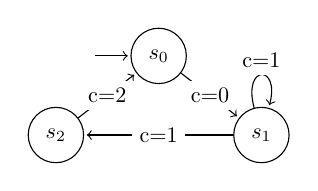
\begin{tikzpicture}[shorten >=1pt,node distance=2cm,/tikz/initial text =, every node/.style={scale=0.8, fill=white}]
    \tikzstyle{every state}=[]
  
    \node[state,initial]   (s)  {$s_0$};
    \node[state] (q_1) [below right=0.5cm and 0.8cm of s]  {$s_1$};
    \node[state] (q_2) [below left=0.5cm and 0.8cm of s] {$s_2$};
  
    \path[->]
    (s)   edge              node {c=0} (q_1)
    (q_1) edge [loop above]  node {c=1} (   )
            edge node {c=1} (q_2)
    (q_2) edge  node {c=2} (s);
  \end{tikzpicture}
\end{center}
  
\label{fig:first_system_example}
\end{minipage}%
\begin{minipage}{0.65\textwidth}
\begin{align*}
&\pi := (c=0)~ (c=1)^\omega,~
\pi' := ((c=0)~ (c=1)~ (c=2))^\omega \\
&\HAssign_1: \{c_\pi \mapsto 0, c_{\pi'} \mapsto 0\}, \HAssign_2 : \{c_\pi \mapsto 1, c_{\pi'} \mapsto 1\} \\
&\HAssign_3: \{c_\pi \mapsto 1, c_{\pi'} \mapsto 2\}, \HAssign_4 : \{c_\pi \mapsto 1, c_{\pi'} \mapsto 0\} \\
\end{align*}
\end{minipage}
\caption{Left: A program automaton. Right: two traces $\pi$ and $\pi'$ of the program automaton. We interpret each trace as a computation. When executing both traces simultaneously, every time point has a corresponding hyper-assignment that assigns values to $c_{\pi}$ and $c_{\pi'}$. Those for the first four time steps are shown on the right. Together, they define the hyper-computation $\HComput := \HAssign_1(\HAssign_2~\HAssign_3~\HAssign_4)^\omega$, matching $\pi$ and $\pi'$.}
\end{figure}

\begin{definition}
     Let  $c_\pi \in \Cells \times \TraceVs, \HPredTerm \in \HPredTerms, \HFuncTerm{} \in \HFuncTerms$. A \emph{HyperTSL(T) formula} is defined by the following grammar:
\begin{align*}
    \varphi &::= \psi~|~\forall \pi.~ \varphi~|~\exists \pi.~\varphi \\
    \psi &::= \HPredTerm~|~\Upd{c_\pi}{\HFuncTerm{}}~|~\neg \psi~| ~\psi\wedge\psi~|~\LTLnext \psi~|~\psi\LTLuntil\psi~
\end{align*}
\end{definition}
To define the semantics of HyperTSL(T), we need the ability to extend a hyper-computation to new trace variables, one for each path quantifier. 
Let $\HComput\in\HAssigns^\omega$ be a hyper-computation, and let
$\pi, \pi' \in \TraceVs, \Comput \in \Assigns^{\omega} $ and $ x \in (\Inputs \cup \Cells)$. We define the extension of $\HComput$ by $\pi$ using the computation $\Comput$ as $ \ExtComput{\HComput}{\pi}{\Comput}~(x_{\pi'})= \HComput(x_{\pi'}) $ for $ \pi' \neq \pi$, and $\ExtComput{\HComput}{\pi}{\Comput}~(x_\pi)= \Comput(x_\pi)$ for $\pi$. 


\begin{definition}
    The \emph{satisfaction of a HyperTSL(T)-Formula} w.r.t. a hyper- computation $\HComput \in \HAssigns^\omega$, a set of computations $\Computs$ and a time point $t$ is defined by
    \begin{align*}
        &t, Z, \HComput \models \forall \pi.~\varphi &&\Leftrightarrow \forall \Comput \in \Computs.~t,~Z,~\ExtComput{\HComput}{\pi}{\Comput} \models \varphi \\
        &t, Z, \HComput \models \exists \pi.~\varphi &&\Leftrightarrow \exists \Comput \in \Computs.~t,~Z,~\ExtComput{\HComput}{\pi}{\Comput} \models \varphi \\
    \end{align*}
    The cases that do not involve path quantification are analogous to those of TSL(T) as defined in Sec.~\ref{prelim:tsl}. We define $Z \models \varphi$ as $0, Z, \emptyset^\omega \models \varphi$.
\end{definition}
%\input{finite_case2}
\label{infinitestuff}


\section{Büchi Product Programs and TSL Model Checking}\label{sec:tslMC}
We now describe how we model the system and specification as Büchi automata, adapting the automata of~\cite{FairnessModTheory} to the setting of TSL. Then, we introduce our model checking algorithm for TSL(T). 
In Sec~\ref{sec:hyperMC} we build on this algorithm to propose an algorithm for HyperTSL(T) model checking. 

We use a symbolic representation of the system (see, for example,~\cite{SoftwareModelCheckingAutomata}), where transitions are labeled with program statements, and all states are accepting. 


\begin{definition}\label{def:grammar} Let $c \in \Cells, \PredTerm \in \PredTerms$ and $\FuncTerm{} \in \FuncTerms$. We define the set of \emph{(basic) program statements} 
as  
\begin{align*}
    s_0 &::= \mathit{assert}(\PredTerm)~|~c:= \FuncTerm{}~|~c:=* \\
    s &::= s_0~|~s;s
\end{align*}
We call statements of the type $s_0$ \emph{basic program statements}, denoted by $\BStmt$; statements of type $s$ are denoted by $\Stmt$. 
The assignment $c:= *$ means that any value could be assigned to $c$.

%\begin{align*}
 %    &s_0 ::= assert(\PredTerm)~|~c:= \FuncTerm{}~|~c:=* \\
 %&s ~::= s_0~|~s;s
 %\end{align*}
\end{definition}

 % - for example, if $c$ is chosen as a random number. 

A \textit{program automaton} $\aut{P}$ is a 
Büchi automaton with $\Sigma = \Stmt$, that is,
$\aut{P} = (\Stmt, Q, q_0, \delta, F)$ and  $\delta \subseteq Q \times \Stmt \times Q$. 
%where $Q$ is a set of program locations; $q_0 \in Q$ is the initial location; $\delta \subseteq Q \times \Stmt \times Q$ is the transition relation; and $F \subseteq Q$ is the set of accepting states. 
When modeling the system we only need basic statements, thus we have $\Stmt = \BStmt$; and $F = Q$ as all states are accepting. See Fig.~\ref{fig:first_system_example} for  an illustration.

Using a program automaton, one can model \verb|if| statements, \verb|while| loops, and non-deterministic choices. However, not every trace of the program automaton corresponds to a program execution. For example, the trace $(n := \mathit{input}_1);\mathit{assert} (n > 0);\mathit{assert}(n < 0);~\mathit{assert}(true)^\omega$ does not -- the second assertion will always fail. Such a trace is called \textit{infeasible}. 
We call a trace \textit{feasible} if it corresponds to a program execution where all the assertions may succeed. We now define this formally.

\begin{definition} \label{def:matches}
    A computation $\Comput$ \emph{matches} a trace $\PTrace \in \BStmt^\omega$ at time point $t$, denoted by $\matchest{\Comput}{\PTrace}{t}$, if the following holds:
    \begin{align*}
        % \begin{cases}
            &\text{if } \PTrace_t = \mathit{assert}(\tau_P):&& \Eval(\PredTerm, \Comput_{t-1}) = true ~\text{ and }~ \forall c \in \Cells.~\Comput_t(c) = \Comput_{t-1}(c)  \\
            &\text{if }\PTrace_t = c:= \FuncTerm{}:&& \Eval(\FuncTerm{}, \Comput_{t-1}) = \Comput_t(c)  ~\text{ and }~ \forall c' \in \Cells \backslash \{c\}.~\Comput_t(c') = \Comput_{t-1}(c')  \\
            &\text{if } \PTrace_t = c := *: && \forall c \in \Cells\backslash\{c\}.~\Comput_t(c) = \Comput_{t-1}(c)
        % \end{cases}
    \end{align*}
    where $\Comput_{-1}$ is the initial assignment.
    A computation $\Comput$ matches a trace $\PTrace \in \BStmt^\omega$, denoted by $\matches{\Comput}{\PTrace}$, if $\forall t \in \mathbb{N}.~\matchest{\Comput}{\PTrace}{t}$.

\end{definition}

\begin{definition}
    A program automaton $\aut{P}$ over $\BStmt$ satisfies a TSL(T)-formula $\varphi$, if for all traces $\PTrace$ of $P$ we have
 $   \forall \Comput \in \Assigns^\omega.~\matches{\Comput}{\PTrace} \Rightarrow \Comput \models \varphi$.
\end{definition}

We now present an algorithm to check whether a program automaton $\aut{P}$ satisfies a TSL(T) formula. It is an adaption of the automaton-based LTL software model checking approach by~\cite{FairnessModTheory}, where the basic idea is to first translate the negated specification $\varphi$ into an automaton $\aut{A}_{\neg \varphi}$, and then combine $\aut{A}_{\neg \varphi}$ and $\aut{P}$ to a new automaton, namely the \textit{Büchi program product}. The program satisfies the specification iff the Büchi program product accepts no feasible trace.

In \cite{FairnessModTheory}, the Büchi program product is constructed similarly to the standard product automata construction. To ensure that the result is again a program automaton, the transitions are not labeled with pairs $(s, \edgel) \in \BStmt \times 2^{AP}$, but with the program statement $(s;~ \mathit{assert}(\edgel))$. A feasible accepted trace of the Büchi program product then corresponds to a counterexample proving that the program violates the specification. In the following, we discuss how we adapt the construction of the Büchi program product for TSL(T) such that this property -- a feasible trace corresponds to a counterexample -- remains true for TSL(T). %Moreover, we want to construct the TSL Büchi program product in such a way that we can use the same algorithm as in \cite{FairnessModTheory} for testing if there is a feasible accepted trace.

Let $\varphi$ be a TSL(T) specification. 
For the construction of $\aut{A}_{\neg \varphi}$, we treat all update and predicate terms as atomic propositions, resulting in an LTL formula $\neg\varphi_{\textit{LTL}}$, which is translated to a Büchi automaton.\footnote{For the translation of LTL formulas to Büchi automata, see, for example,~\cite{LTL_Buechi, LTL_Buechi2, LTL_Buechi_Tut}.} 
 For our version of the Büchi program product, we need to merge a transition label $s$ from $\aut{P}$
 with a transition label $\edgel$ from $\aut{A}_{\neg\varphi_{\textit{LTL}}}$ into a single program statement such that the assertion of the combined statement succeeds iff $\edgel$ holds for the statement $s$. Note that $\edgel$ is a set of update and predicate terms. For the update terms $\Upd{c}{\FuncTerm{}}$ we cannot just use an assertion to check if they are true, as we need to `save' the value of $\FuncTerm{}$ before the statement $s$ is executed.

Our setting differs from~\cite{FairnessModTheory} also in the fact that their program statements~do not reason over input streams. We model the behavior of input streams by using fresh memory cells that are assigned a new value at every time step.  
In the following, we define a function $\mathit{combine} $ that combines a program statement $s$ and a transition label $\edgel$ to a new program statement as described above.
%Now, we combine $A_{\neg \varphi}$ with the program automaton to create the Büchi program product, whose feasible traces correspond to feasible traces of the program automaton that do not satisfy the TSL formula. The construction is similar to that of a product automaton, but is defined in such a way that the Büchi program product is again a program automaton. To achieve that, 
\begin{definition}
Let $\USet = \{\Upd{c_1}{\FuncTerm{1}}, \dots, \Upd{c_n}{\FuncTerm{n}}\}$ be the set of update terms appearing in $\varphi$, let $\PredSet$ be the set of predicate terms appearing in $\varphi$. Let $\edgel \subseteq (\USet \cup \PredSet)$ be a transition label of $\aut{A}_{\neg \varphi}$.  Let $(tmp_j)_{j \in \mathbb{N}}$ be a family of fresh cells. Let $\Inputs = \{i_1, \dots i_m \}$. We define the function $\mathit{combine} : \Stmt \times \mathcal{P}(\PredTerms \cup \UpdTerms) \rightarrow \Stmt$ as follows. The result of $\combine{s}{\edgel}$ is composed of the program statements in $\mathit{save\_values}_\edgel, s, \mathit{new\_inputs}, \mathit{check\_preds}_\edgel$ and $\mathit{check\_updates}_\edgel$. Then we have: 
\begin{align*}
    \mathit{save\_values} &:= \mathit{tmp}_1 := \FuncTerm{1};~\dots ;\mathit{tmp}_n := \FuncTerm{n} \\
    \mathit{new\_inputs} &:= i_1 := *;~\dots~; i_m := *\\
    \mathit{check\_preds}_\edgel &:= assert \left(\bigwedge_{\PredTerm \in \edgel} \PredTerm \wedge \bigwedge_{\PredTerm \in \PredSet \backslash \edgel} \neg \PredTerm \right) \\
    \mathit{check\_updates}_\edgel &:= assert \left( \bigwedge_{\Upd{c_j}{\FuncTerm{j}} \in \USet}
    \begin{cases}
        c_j = \mathit{tmp}_j &\text{if } \Upd{c_j}{\FuncTerm{j}} \in \edgel\\
        c_j \neq \mathit{tmp}_j &\text{else} 
    \end{cases}        
        \right) \\
    \combine{s}{\edgel} &:= \mathit{save\_values};~s;~\mathit{new\_inputs};~\mathit{check\_preds}_\edgel;~\mathit{check\_updates}_\edgel
\end{align*}
\end{definition}

We can extend this definition to combining traces instead of single transition labels. 
%a program trace and a predicate trace by applying it per timepoint. 
This leads to a function $\mathit{combine} : \Stmt^\omega \times \mathcal{P}(\PredTerms \cup \UpdTerms)^\omega \rightarrow \Stmt^\omega$.
Note that the result of $\mathit{combine}$ is again a program statement in $\Stmt$ (or a trace $\Stmt^\omega$) over the new set of cells $\Cells \cup \Inputs \cup (tmp_j)_{j \in \mathbb{N}}$, which we call $\Cells^*$.

\begin{example}
    Let $\Inputs = \{i\}$. Then the result of $\combine{n := 42}{ \{ \Upd{n}{n + 7}, n > 0\}} $ is $\mathit{tmp}_0 := n + 7;~n := 42;~i := *;~ \mathit{assert} (n > 0);~ \mathit{assert} (n = \mathit{tmp}_0)$.
\end{example}

As $\mathit{combine}$ leads to composed program statements, we now need to extend the definition of feasibility to all traces. To do so, we define a function $\mathit{flatten}: \Stmt^\omega \rightarrow {\Stmt_0}^\omega$ that takes a sequence of program statements and transforms it into a sequence of basic program statements by converting a composed program statement into multiple basic program statements.

\begin{definition}
    A trace $\PTrace \in \Stmt^\omega$ \emph{matches} a computation $\Comput$, denoted by $\matches{\Comput}{\PTrace}$ if $\matches{\Comput}{\flatten{\PTrace}}$.
    A trace $\PTrace$ is \emph{feasible} if there is a computation $\Comput$ such that $\matches{\Comput}{\PTrace}$.
\end{definition}

\begin{definition}{\textbf{(Combined Product)}} 
    Let $\aut{P} = (Stmt, Q, q_0, \delta, Q)$ be a program automaton and $\aut{A} = (\mathcal{P}(\PredTerms \cup \UpdTerms), Q', q_0', \delta',F')$ be a Büchi automaton (for example, the automaton $\aut{A}_{\neg \varphi_{LTL}}$). The combined product $\aut{P} \BuechiProd \aut{A}$ is an automaton $\aut{B} = (Stmt, Q \times Q', (q_0, q_0'), \delta_B, F_{B})$, where 
    \begin{align*}
        F_{B} &= \{(q, q') \mid q \in Q \wedge q' \in F'\} \\
        \delta_B &= \{((p, q), \combine{s}{\edgel}, (p', q'))~|~(p, s, p') \in \delta \wedge (q, \edgel, q') \in \delta'\}
    \end{align*}
\begin{comment}  
\begin{itemize}
    \item $\delta_B = \{((p, q), \combine{s}{\edgel}, (p', q'))~|~(p, s, p') \in \delta \wedge (q, \edgel, q') \in \delta'\}$, and
    \item $ F_{B} = \{(q, q') \mid q \in Q \wedge q' \in F'\}$
\end{itemize}
\end{comment}
\end{definition}

\begin{theorem} \label{thm:BuechiProdModelChecking}
    Let $\aut{P}$ be a program automaton over $\BStmt$. Let $\varphi$ be a TSL(T) formula. Then $\aut{P}$ satisfies $\varphi$ if and only if $\aut{P} \BuechiProd \aut{A}_{\neg \varphi_{LTL}}$ has no feasible trace.
\end{theorem}

\begin{proof}[sketch]
    If $\matches{\Comput}{\sigma}$ is a counterexample, we can construct a computation $\tilde\Comput$ that matches the corresponding combined trace in $\aut{P} \BuechiProd \aut{A}_{\neg \varphi_{LTL}}$, and vice versa. The formal construction is given in App.~\ref{sec:buechi_corr}. 
\end{proof}


%The main idea of the proof is a construction that, given a computation that matches a program trace and violates $\varphi$, constructs a computation matching the combined trace and vice versa. For more details, see App. \ref{sec:buechi_corr}.

We can now apply Thm. \ref{thm:BuechiProdModelChecking} to solve the model checking problem by testing whether $\aut{P} \BuechiProd \aut{A}_{\neg \varphi_{LTL}}$ does not accept any feasible trace, using the feasibility check in~\cite{FairnessModTheory} as a black box. 
%After generating the combined product, we can use the algorithm of~\cite{FairnessModTheory}, which tests if a feasible trace exists. 
The algorithm of~\cite{FairnessModTheory} is based on counterexample-guided abstraction refinement (CEGAR \cite{CEGAR}). Accepted traces are checked for feasibility.  
%when a trace that is accepted by the automaton is found, the trace is checked for feasibility. 
First, finite prefixes of the trace are checked using an SMT-solver. If they are feasible, a ranking function synthesizer is used to check whether the whole trace eventually terminates. If the trace is feasible, it serves as a counterexample. If not, the automaton is refined such that it now does not include the spurious counterexample trace anymore, and the process is repeated. For more details, we refer to \cite{FairnessModTheory}. 
The limitations of SMT-solvers and ranking function synthesizers also limit the functions and predicates that can be used in both the program and in the TSL(T) formula. 


\section{HyperTSL(T) Model Checking}
We now turn to the model checking problem of HyperTSL(T). We start with alternation-free formulas and continue with $\forall^*\exists^*$ formulas. 

\subsection{Alternation-free HyperTSL(T)}\label{sec:altfree}

In this section, we apply the technique of self-composition to extend the algorithm of Sec.~\ref{sec:tslMC} to alternation-free HyperTSL(T).
%, similarily to Section \ref{sec:FiniteHyper}, but now for a program automaton. 
%Self-composition is a technique commonly used for the verification of hyperproperties \cite{SelfComposition1, SelfComposition2, SelfComposition3}.
%\subsection{The Algorithm}
First, we define what it means for a program automaton to satisfy a HyperTSL(T) formula.

\begin{definition}
    Let $\aut{P}$ be a program automaton over $\BStmt$, let $\varphi$ be a HyperTSL(T) formula and let $Z=\{\Comput \in \Assigns^\omega ~|~ \exists \PTrace.~\matches{\Comput}{\PTrace} \text{ and } \PTrace \text{ is a trace of }\aut{P} \}$. 
    We say that $\aut{P}$ \emph{satisfies} $\varphi$ if $Z \models \varphi$.
\end{definition}

\begin{definition}
    Let $\aut{P} = (\Stmt, Q, q_0, \delta, Q)$ be a program automaton. The \emph{$n$-fold self-composition} of $\aut{P}$ is $\aut{P}^n = (\Stmt', Q^n, q_0^n, \delta^n, Q^n)$, where $\Stmt'$ are program statements over the set of inputs $\Inputs \times \TraceVs$ and the set of cells $\Cells \times \TraceVs$ and where $Q^n = Q \times \dots \times Q$,  $q_0^n = (q_0, \dots , q_0)$ and
    \begin{align*}
        \delta^n = &\{((q_1, \dots, q_n), ((s_1)_{\pi_1}; \dots; (s_n)_{\pi_n}), (q_1', \dots, q_n')) \\
        & \quad \mid \forall 1 \leq i \leq n.~ (q_i, s_i, q_i') \in~\delta\}
    \end{align*}
where $(s)_{\pi}$ renames every cell $c$ used in $s$ to $c_{\pi}$ and every input $i$ to $i_{\pi}$.
\end{definition}

\begin{theorem} \label{thm:BuechiProdModelCheckingAFH}
    A program automaton $\aut{P}$ over $\BStmt$ satisfies a universal HyperTSL(T) formula $\varphi = \forall \pi_1.~ \dots \forall \pi_n.~\psi$ iff $\aut{P}^n \BuechiProd \aut{A}_{\neg \psi_{LTL}}$ has no feasible trace.
\end{theorem}

\begin{theorem} \label{thm:BuechiProdModelCheckingAFH2}
    A program automaton $P$ over $\BStmt$ satisfies an existential HyperTSL(T) formula $\varphi = \exists \pi_1.~ \dots \exists \pi_n.~\psi$ iff $\aut{P}^n \BuechiProd \aut{A}_{\psi_{LTL}}$ has some feasible trace.
\end{theorem}

\noindent The proofs of are analogous to the proof of Thm.~\ref{thm:BuechiProdModelChecking} and are provided in~App.~\ref{sec:BuechiProd_corr2}.
\subsection{ $\forall^* \exists^*$ HyperTSL(T)}\label{sec:hyperMC}

In this section, we present a sound but necessarily incomplete algorithm for finding counterexamples for $\forall^* \exists^*$ HyperTSL(T) formulas.\footnote{Note that the algorithms of Sec.~\ref{sec:tslMC} and Sec.~\ref{sec:altfree} are also incomplete, due to the feasibility test. However, the incompleteness of the algorithm we provide in this section is inherent to the quantifier alternation of the formula.}
%there is also for HyperLTL no such algorithm yet, thus this also gives the first software model checking algorithm for finding counterexamples for $\forall^* \exists^*$ HyperLTL formulas. 
Such an algorithm %that finds counterexamples for the $\forall^* \exists^*$ fragment 
can also provide witnesses $\exists^* \forall^*$ formulas. As HyperTSL(T) is built on top of HyperLTL, we combine ideas from finite-state HyperLTL model checking~\cite{HyperLTLModelChecking}
with the algorithms of Sec.~\ref{sec:tslMC} and Sec.~\ref{sec:altfree}.

Let $\varphi = \forall^m \exists^n. \psi$. For HyperLTL model checking, \cite{HyperLTLModelChecking} first constructs an automaton containing the system traces satisfying $\psi_\exists := \exists ^n. \psi$, and then applies complementation to extract counterexamples for the $\forall\exists$ specification.
Consider the automaton $\aut{P}^n \BuechiProd \aut{A}_{\psi_{LTL}}$ from Sec.~\ref{sec:tslMC}, whose feasible traces correspond to the system traces satisfying $\psi_\exists$. If we would be able to remove all infeasible traces, we could apply the finite-state HyperLTL model checking construction.
Unfortunately, removing all infeasibilities is impossible in general, as the result would be a finite-state system describing exactly an infinite-state system. Therefore, the main idea of this section is to remove parts of the infeasible traces from $\aut{P}^n \BuechiProd \aut{A}_{\psi_{LTL}}$, constructing an over-approximation of the system traces satisfying $\psi_\exists$. 
A counterexample disproving $\varphi$ is then a combination of system traces that is not contained in the over-approximation. 

We propose two techniques for removing infeasibility. The first technique removes \textit{k-infeasibility} from the automaton, that is, a local inconsistency in a trace, occurring within $k$ consecutive time steps. When choosing $k$, there is a tradeoff: if $k$ is larger, more counterexamples can be identified, but the automaton construction gets exponentially larger. 

The second technique removes \textit{infeasible accepting cycles} from the automaton. It might not be possible to remove all of them, thus we bound the number of iterations. We present an example and then elaborate on these two methods. 


\begin{example}
    The trace $t_1$ below is 3-infeasible, because regardless of the value of $n$ prior to the second time step, the assertion in the fourth time step will fail.
    %\begin{align*}
     $$   t_1 = (n--;~ \mathit{assert}(n >= 0))~ (n:= 1;~ \mathit{assert} (n >= 0))~ (n--;~ \mathit{assert} (n >= 0))^\omega $$
    %\end{align*}
    In contrast, the trace 
    $t_2 = (n := *)~(n--;~ \mathit{assert} (n >= 0))^\omega$
    is not $k$-infeasible for any $k$, because the value of $n$ can always be large enough to pass the first $k$ assertions. Still, the trace is infeasible because $n$ cannot decrease forever without dropping below zero. If such a trace is accepted by an automaton, $n--;~\mathit{assert} (n >= 0)$ corresponds to an infeasible accepting cycle.    
\end{example}

\subsubsection{Removing $k$-infeasibility} 
 To remove $k$-infeasibility from an automaton, we  construct a new program automaton that `remembers' the $k-1$ previous statements. The states of the new automaton correspond to paths of length $k$ in the original automaton. We add a transition labeled with $l$ between two states $p$ and $q$ if we can extend the trace represented by $p$ with $l$ such that the resulting trace is $k$-feasible. Formally, we get: 


\begin{definition}
    Let $k \in \mathbb{N}$, $\PTrace \in \Stmt^\omega$. We say that $\PTrace$ is \emph{$k$-infeasible} if there exists $j \in \mathbb{N}$ such that $\PTrace_j \PTrace_{j+1} \dots \PTrace_{j+k-1}; \mathit{assert}(true)^\omega$ is infeasible for all possible initial assignments $\Comput_{-1}$. We then also call the subsequence $\PTrace_{j}\PTrace_{j+1}\dots \PTrace_{j+k-1}$ infeasible.
    If a trace is not $k$-infeasible, we call it $k$-feasible.\footnote{Whether a subsequence $\PTrace_j\PTrace_{j+1} \dots \PTrace_{j+k-1}$ is a witness of k-infeasibility can be checked using an SMT-solver, e.g, \cite{Z3, SMT1, SMT2, SMT3}.}
\end{definition}



\begin{definition}
    Let $\aut{P} = (\Stmt, Q, q_0, \delta, F)$ be a program automaton. Let $k \in \mathbb{N}$. We define $\aut{P}$ without $k$-infeasibility, as $\aut{P}_k = (\Stmt, Q', q_0, \delta', F')$ where
    \begin{align*}
        Q' :=& \{(q_1,s_1,q_2 \dots ,s_{k-1},q_k) \mid (q_1, s_1, q_2) \in \delta \wedge \dots \wedge (q_{k-1}, s_{k-1}, q_k) \in \delta \}~ \cup \\
        &\{(q_0, s_0,q_1 \dots ,s_{k' - 1}, q_{k'}) \mid k' < k-1 \wedge (q_0, s_0, q_1) \in \delta \wedge \dots \\
        & \phantom{(q_0, s_0,q_1 \dots ,s_{k' - 1}, q_{k'}) \mid} \quad \wedge (q_{k'-1}, s_{k'-1}, q_{k'}) \in \delta  \} \\
        \delta' :=& \{((q_1,s_1,q_2\dots ,s_{k-1},q_k), s_k, (q_2,s_2, \dots ,q_k,s_k,q_{k+1})) \in Q' \times \Stmt \times Q' \\ &\quad \mid s_1 \dots s_k \text{ feasible} \}~\cup \\
        &\{((q_0,s_0,q_1\dots ,s_{k'-1},q_{k'}), s_{k'}, (q_0, s_0, \dots ,q_{k'},s_{k'},q_{k'+1})) \in Q' \times \Stmt \times Q' \\ &\quad \mid k' < k-1 \wedge s_0 \dots s_{k'} \text{ feasible} \} \\
        F' :=& \{(q_1,s_1,q_2 \dots ,s_{k-1},q_k) \in Q' \mid q_k \in F \}~\cup \\
        & \{(q_0, s_0,q_1 \dots ,s_{k' - 1}, q_{k'}) \in Q' \mid k' < k-1 \wedge q_{k'} \in F\}
    \end{align*}
\end{definition}

\begin{theorem} \label{thm:k_feasible}
   $\aut{P}_k$ accepts exactly the $k$-feasible traces of~$\aut{P}$.
\end{theorem}
The proof follows directly from the construction above, see App.~\ref{sec:k_feasible_proof} for details. 

\subsubsection{Removing Infeasible Accepting Cycles} 
For removing infeasible accepting cycles, we first enumerate all simple cycles of the automaton (using, e.g.,~\cite{CycleFinding}), adding also cycles induced by self-loops. For each cycle $\varrho$ that contains at least one accepting state, we test its feasibility: first, using an SMT-solver to test if $\varrho$ is locally infeasible; then, using a ranking function synthesizer (e.g., \cite{Termination1, Termination2, Termination3}) to test if $\varrho^\omega$ is infeasible. If we successfully prove infeasibility, we refine the model, using the methods from \cite{SoftwareModelCheckingAutomata, TerminationRefinement}. This refinement is formalized in the following.


\begin{definition}
    Let $\aut{P}=(\Stmt, Q, q_0, \delta, F)$ be a program automaton. Let $\varrho = (q_1, s_1, q_2)(q_2, s_2, q_3)\dots(q_n, s_n, q_1)$ be a sequence of transitions of $\aut{P}$. We say that~$\varrho$ is an \emph{infeasible accepting cycle} if there is a $1 \leq j \leq n$ with $q_j \in F$ and $(s_1 s_2 \dots s_{n-1})^\omega$ is infeasible for all possible initial assignments $\Comput_{-1}$.
\end{definition}

\begin{definition}
    Let $\aut{P}$ be a program automaton and $C \subseteq (Q \times \Stmt \times Q)^\omega$ be a set of infeasible accepting cycles of $\aut{P}$.
    Furthermore, let
    $$\varrho = (q_1, s_1, q_2)(q_2, s_2, q_3)\dots(q_{n-1}, s_{n-1}, q_n) \in~C.$$
    The automaton $\aut{A}_\varrho$ for $\varrho$ is $ \aut{A}_\varrho = (\Stmt, Q=\{q_0, q_1, \dots q_n\}, q_0, \delta, Q \backslash \{q_0 \}) $ where 
   \begin{align*}
        \delta ~=~ &\{(q_0, s, q_0) \mid s \in \Stmt \} \\
        & \cup \{(q_j, s_j, q_{j+1}) \mid 1 \leq j < n \} \cup \{(q_0, s_1, q_2), (q_n, s_n, q_1)\}.
   \end{align*}
    \end{definition}
   Then, $\aut{A}_\varrho$ accepts exactly the traces that end with $\varrho^\omega$, without any restriction on the prefix. See Fig. \ref{fig:aut_infeasible_cycle} for an example. To exclude the traces of $\aut{A}_\varrho$ from $\aut{P}$, we define
    $
        \aut{P}_C := \aut{P} \backslash \left( \bigcup_{\varrho \in C} \aut{A}_\varrho \right)
    $.\footnote{For two automata $\aut{A}_1, \aut{A}_2$ we use $\aut{A}_1 \backslash \aut{A}_2$ to denote the intersection of $\aut{A}_1$ with the complement of $\aut{A}_2$, resulting in the language $\aut{L}(\aut{A}_1) \setminus\aut{L}(\aut{A}_2)$. }
    This construction can be repeated to exclude infeasible accepted cycles that are newly created in $\aut{P}_C$. We denote the result of iterating this process $k'$ times by~$\aut{P}_{C(k')}$.

\subsubsection{Finding Counterexamples for $\forall^* \exists^*$ HyperTSL(T)-Formulas} 
Consider now a HyperTSL(T) formula $\varphi = \forall^{1\cdots m}\exists ^{m+1\cdots n}.\psi$ and a program automaton $\aut{P}$.
\begin{wrapfigure}{r}{0.5\textwidth}
    \vspace{-1cm}
    \begin{center}
    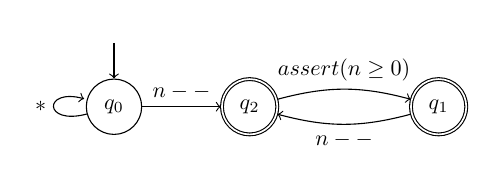
\begin{tikzpicture}[node distance= 3cm, /tikz/initial text =, every node/.style={scale=0.8}]
        \node[state, initial above] (s0) {$q_0$};
        \node[state, accepting] (s2) [right=1cm of s0] {$q_2$};
        \node[state, accepting] (s1) [right of=s2] {$q_1$};

        \path[->]
        (s0) edge [loop left] node {$*$} ( )
            edge [above] node {$n--$} (s2)
        (s1) edge [bend left = 15, below] node {$n--$} (s2)
        (s2) edge [bend left = 15, above] node {$assert(n \geq 0)$} (s1);
    
    \end{tikzpicture}
    \end{center}
    \vspace{-5mm}
    \caption{Automaton $\aut{A}_{\varrho}$ for the infeasible cycle
    $\varrho = (q_1,~n--,~q_2)(q_2,~ assert(n>0),~ q_1)$. Label $*$ denotes an edge for every (relevant) statement.}
    \label{fig:aut_infeasible_cycle}
    \vspace{-1cm}
\end{wrapfigure}
For finding a counterexample, we first construct the combined product $\aut{P}^n \BuechiProd \aut{A}_\psi$. 
Each feasible accepted trace of $\aut{P}^n \BuechiProd \aut{A}_\psi$ corresponds to a combination of $n$ feasible program traces that satisfy $\psi$. Next, we eliminate $k$-infeasibility and remove $k'$-times infeasible accepting cycles from the combined product, resulting in the automaton $(\aut{P}^n \BuechiProd \aut{A}_\psi)_{k, C(k')}$. Using this modified combined product, we obtain an over-approximation of the program execution combinations satisfying the existential part of the specification.
 Each trace of the combined product is a combination of $n$ program executions and a predicate/update term sequence. We then project the $m$ universally quantified program executions from a feasible trace, obtaining a tuple of $m$ program executions that satisfy the existential part of the formula. Applying this projection to all traces of $(\aut{P}^n \BuechiProd \aut{A}_\psi)_{k, C(k')}$ leads to an over-approximation of the program executions satisfying the existential part of the specification. Formally:

\begin{definition}
    Let $\aut{P}$ be a program automaton, let $m\leq n \in \mathbb{N}$, and let $\aut{A}_\psi$ be the automaton for the formula $\psi$. Let $(\aut{P}^n \BuechiProd \aut{A})_{k, C(k')} = (\Stmt, Q, q_0, \delta, F)$. We define the \emph{projected automaton} $(\aut{P}^m \BuechiProd \aut{A})_{k, C(k')}^\forall = (\Stmt, Q, q_0, \delta^\forall, F)$ where
    %\begin{align*}
 $   \delta^\forall = \{(q, (s_1; \dots ;~s_m), q') \mid \exists s_{m+1}, \dots s_n, \edgel.~ (q, \combine{s_1; \dots ;~s_n}{\edgel},q') \in \delta \} $.
 %\footnote{Recall that $s_1;s_2$ refers to a sequence of statements, as given in Def.~\ref{def:grammar}. For more details on the universal projection we refer the reader to\cite{DBLP:conf/fsttcs/FinkbeinerP22}.}
    %\end{align*}
\end{definition}
The notation $s_1;s_2$ refers to a sequence of statements, as given in Def.~\ref{def:grammar}. For more details on the universal projection we refer the reader to\cite{DBLP:conf/fsttcs/FinkbeinerP22}.

Now, it only remains to check whether the over-approximation contains all tuples of $m$ feasible program executions. If not, a counterexample is found. This boils down to testing if $\aut{P}^m \backslash (\aut{P}^n \BuechiProd \aut{A}_\psi)_{k, C(k')}^\forall$ has some feasible trace.
 Thm.~\ref{thm:corr_AE} states the soundness of our algorithm. See App.~\ref{sec:corr_AE} for its proof. 

\begin{theorem} \label{thm:corr_AE}
    Let $\varphi = \forall^{1\cdots m}\exists ^{m+1\cdots n}. \psi $ be a HyperTSL(T) formula. If the automaton $\aut{P}^m \backslash (\aut{P}^n \BuechiProd \aut{A}_\psi)_{k, C(k')}^\forall$ has a feasible trace, then $\aut{P}$ does not satisfy $\varphi$.
\end{theorem}




\section{Demonstration of the Algorithm} \label{sec:HyperExamples}

In this section, we apply the algorithm of Sec.~\ref{sec:hyperMC} to two simple examples, demonstrating that removing some infeasibilities can already be sufficient for identifying counterexamples.

\subsubsection{Generalized Noninterference}
Recall the formula $\varphi_{gni} = \forall \pi.~\exists \pi'.~\LTLglobally(i_{\pi'} = \lambda \wedge c_\pi = c_{\pi'})$ introduced in Sec.~\ref{sec:intro}, specifying generalized noninterference. 
We model-check $\varphi_{gni}$ on the program automaton $\aut{P}$ of Fig.~\ref{fig:gni_example_2} (left), setting $\lambda = 0$.
The program $\aut{P}$ violates $\varphi_{gni}$ since for the trace $(assert (i < 0)~ c:=0)^\omega$ there is no other trace where on which $c$ is equal, but $i=0$.
%$P^2$ is shown in Fig.~\ref{fig:gni_example_2}. 

\begin{figure}[t]
\begin{minipage}{0.25\textwidth}
\begin{center}
\begin{tikzpicture}[node distance = 1.5cm,  /tikz/initial text =,every node/.style={scale=0.8}]
    \node[state, initial left, accepting] (s0) {$q_0$};
    \node[state, accepting] (s1) [above of=s] {$q_1$};
    \node[state, accepting] (s2) [below of=s] {$q_2$};

    \path[->]
    (s0) edge [bend left=70] node [fill=white] {$A(i < 0)$} (s1)
        edge [bend right=70] node  [fill=white] {$A(i \geq 0)$} (s2)
    (s1) edge [bend left=70] node [fill=white] {$c := 0$} (s0)
    (s2) edge [bend right=70] node [fill=white] {$c := 1$} (s0);
    
\end{tikzpicture}
\end{center}
\end{minipage}%
\hfill
\begin{minipage}{0.74\textwidth}
\begin{center}
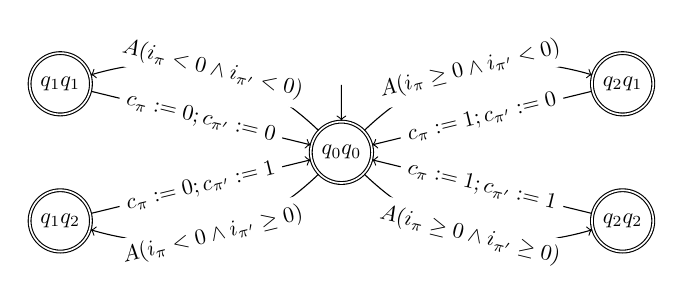
\begin{tikzpicture}[ node distance = 4cm, /tikz/initial text =, every node/.style={scale=0.8, fill=white} ]
    \node[state, initial above, accepting] (s00) {$q_0q_0$};
    \node[state, accepting] (s11) [above left=0.3cm and 3cm of s00] {$q_1q_1$};
    \node[state, accepting] (s12) [below left=0.3cm and 3cm of s00] {$q_1q_2$};
    \node[state, accepting] (s21) [above right=0.3cm and 3cm of s00] {$q_2q_1$};
    \node[state, accepting] (s22) [below right=0.3cm and 3cm of s00] {$q_2q_2$};

    \path[->]
    (s00) edge [bend right=30,sloped] node {$A(i_\pi < 0 \wedge i_{\pi'} < 0)$} (s11)
        edge [bend right=30, sloped] node {$A(i_\pi \geq 0 \wedge i_{\pi'} \geq 0)$} (s22)
        edge [bend left=30, sloped] node {$A(i_\pi \geq 0 \wedge i_{\pi'} < 0 )$} (s21)
        edge [bend left =30, sloped] node {$A(i_\pi < 0 \wedge i_{\pi'} \geq 0)$} (s12)
    (s11) edge [sloped] node {$c_\pi := 0; c_{\pi'} := 0$} (s00)
    (s22) edge [sloped] node {$c_\pi := 1; c_{\pi'} := 1$} (s00)
    (s21) edge [sloped] node {$c_\pi := 1; c_{\pi'} := 0$} (s00)
    (s12) edge [sloped] node {$c_{\pi} := 0; c_{\pi'} := 1$} (s00);
    
\end{tikzpicture}
\end{center}
\end{minipage}
\caption{Left: The program automaton $\aut{P}$ used in the first example. Right: The program automaton $\aut{P}^2$. For brevity, we use $A$ for $assert$ and join consecutive assertions. }
\label{fig:gni_example_2}
\end{figure}

The automaton for $\psi = \LTLglobally(i_{\pi'} = 0 \wedge c_\pi = c_{\pi'})$ consists of a single accepting state with the self-loop labeled with $\PredTerm = (i_{\pi'} = 0 \wedge c_{\pi} = c_{\pi'})$. For this example, it suffices to choose $k=1$. To detect $1$-inconsistencies we construct $\aut{P}^2$ (Fig~\ref{fig:gni_example_2}, right). Then, $(\aut{P}^2 \BuechiProd \aut{A}_{\psi})_k$ is the combined product with all
 $1$-inconsistent 
 \begin{wrapfigure}{r}{0.5\textwidth}
\vspace{-3mm}
\begin{center}
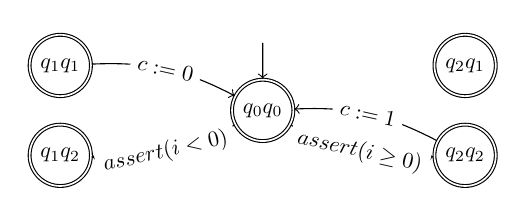
\begin{tikzpicture}[node distance = 5cm, /tikz/initial text = ,every node/.style={scale=0.8, fill=white}]
    \node[state, initial above, accepting] (s00) {$q_0q_0$};
    \node[state, accepting] (s11) [above left=0cm and 2cm of s00] {$q_1q_1$};
    \node[state, accepting] (s12) [below left=0cm and 2cm of s00] {$q_1q_2$};
    \node[state, accepting] (s21) [above right=0cm and 2cm of s00] {$q_2q_1$};
    \node[state, accepting] (s22) [below right=0cm and 2cm of s00] {$q_2q_2$};

    \path[->]
    (s00) edge [bend right=15, sloped] node {$assert(i\geq 0)$} (s22)
        edge [bend left =15, sloped] node {$assert(i < 0)$} (s12)
    (s11) edge [bend left=15, sloped] node {$c:= 0$} (s00)
    (s22) edge [bend right=15, sloped] node {$c:= 1$} (s00);
    
\end{tikzpicture}
\end{center}
\caption{program automaton $(\aut{P}^2 \BuechiProd \aut{A}_{\psi})_k^\forall$}
\label{fig:gni_example_4}
\vspace{-3mm}
\end{wrapfigure}
 transitions removed (see Fig.~\ref{fig:gni_example_3} for the combined product). 


\begin{figure}[t]
\begin{center}
    \tikzset{ every node/.style={scale=0.8, fill=white}}
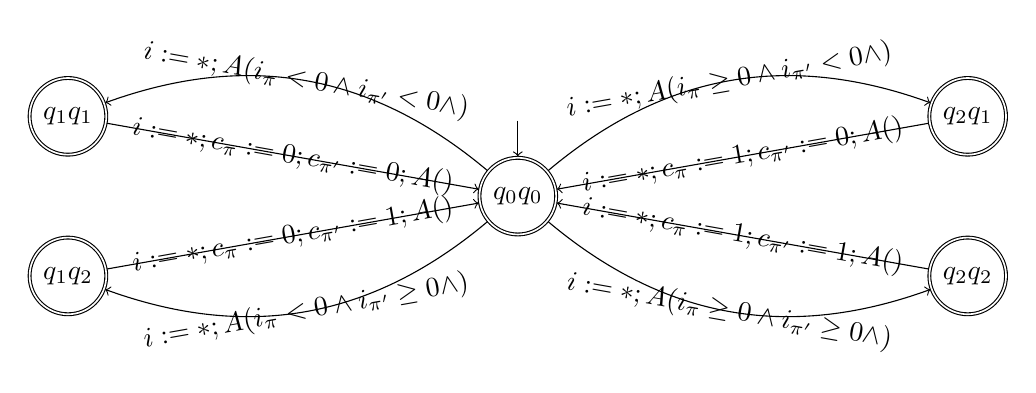
\begin{tikzpicture}[node distance = 5cm, /tikz/initial text = ]
    \node[state, initial above, accepting] (s00) {$q_0q_0$};
    \node[state, accepting] (s11) [above left=0.3cm and 5cm of s00] {$q_1q_1$};
    \node[state, accepting] (s12) [below left=0.3cm and 5cm of s00] {$q_1q_2$};
    \node[state, accepting] (s21) [above right=0.3cm and 5cm of s00] {$q_2q_1$};
    \node[state, accepting] (s22) [below right=0.3cm and 5cm of s00] {$q_2q_2$};

    \path[->]
    (s00) edge [bend right=30, sloped] node {$i := *; A(i_\pi < 0 \wedge i_{\pi'} < 0 \wedge \PredTerm)$} (s11)
        edge [bend right=30, sloped] node {$i := *; A(i_\pi \geq 0 \wedge i_{\pi'} \geq 0 \wedge \PredTerm)$} (s22)
        edge [bend left=30, sloped] node {$i := *;A(i_\pi \geq 0 \wedge i_{\pi'} < 0 \wedge \PredTerm)$} (s21)
        edge [bend left =30, sloped] node {$i := *;A(i_\pi < 0 \wedge i_{\pi'} \geq 0 \wedge \PredTerm)$} (s12)
    (s11) edge [sloped] node {$i := *; c_\pi := 0; c_{\pi'} := 0; A(\PredTerm)$} (s00)
    (s22) edge [sloped] node {$i := *; c_\pi := 1; c_{\pi'} := 1; A(\PredTerm)$} (s00)
    (s21) edge [sloped] node {$i := *;c_\pi := 1; c_{\pi'} := 0; A(\PredTerm)$} (s00)
    (s12) edge [sloped] node {$i := *;c_{\pi} := 0; c_{\pi'} := 1; A(\PredTerm)$} (s00);
    
\end{tikzpicture}
\end{center}
\caption{The combined product $(\aut{P}^2 \BuechiProd \aut{A}_{\psi})$}
\label{fig:gni_example_3}
\end{figure}

The automaton $(\aut{P}^2 \BuechiProd \aut{A}_{\psi})_k^\forall$ is shown in Fig.~\ref{fig:gni_example_4}. 
It does not contain the trace $\sigma = \mathit{assert}(i < 0)~(c:=0)^\omega$ which is a feasible trace of $\aut{P}$. Therefore, $\sigma$ is a feasible trace accepted by $\aut{P}\backslash (\aut{P}^2 \BuechiProd \aut{A}_{\psi})_k^\forall$ and is a counterexample proving that $\aut{P}$ does not satisfy generalized noninterference -- there is no feasible trace that agrees on the value of the cell $c$ but has always $i=0$. %For this example, it is not necessary to remove infeasible cycles.

\subsubsection{The Need of Removing Cycles} 

We now present an example in which removing $k$-infeasibility is not sufficient, but removing infeasible accepting cycles leads to a counterexample. Consider the specification
$
    \varphi = \forall \pi\exists \pi'.\LTLglobally (p_\pi \neq p_{\pi'} \wedge n_\pi < n_{\pi'})
$
and the program automaton $\aut{P}_{cy}$ of Fig. \ref{fig:cycle_example_1}.
The formula $\varphi$ states that for every trace $\pi$, there is another trace $\pi'$ which differs from $\pi$ on $p$, but in which $n$ is always greater. The trace $\pi = (n:= *); (p := *); \mathit{assert}(p = 0); (n--)^\omega$ is a counterexample for $\varphi$ in $\aut{P}_{cy}$  as any trace $\pi'$ which differs on $p$ will decrease its $n$ by $2$ in every time step, and thus $n_{\pi'}$ will eventually drop below $n_\pi$.




\begin{figure}[t]
\begin{minipage}{0.19\textwidth}
\begin{center}
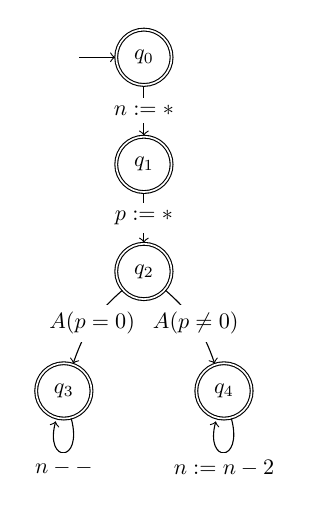
\begin{tikzpicture}[node distance = 1.7cm, /tikz/initial text =, every node/.style={scale=0.8, fill=white}]
    \node[state, initial, accepting] (s0) {$q_0$};
    \node[state, accepting] (s1) [below of=s0] {$q_1$};
    \node[state, accepting] (s2) [below of=s1] {$q_2$};
    \node[state, accepting] (s3) [below left= 1cm and 0.5cm of s2] {$q_3$};
    \node[state, accepting] (s4) [below right=1cm and 0.5cm of s2] {$q_4$};

    \path[->]
    (s0) edge node {$n := *$} (s1)
    (s1) edge node {$p := *$} (s2)
    (s2) edge [bend right=15] node {$A(p = 0)$} (s3)
    (s2) edge [bend left=15] node {$A(p \neq 0)$}  (s4)
    (s3) edge [loop below] node {$n--$} ( )
    (s4) edge [loop below] node {$n := n-2$} ( );
    
\end{tikzpicture}
\end{center}
\end{minipage}%
\hfill
\begin{minipage}{0.79\textwidth}
\begin{center}
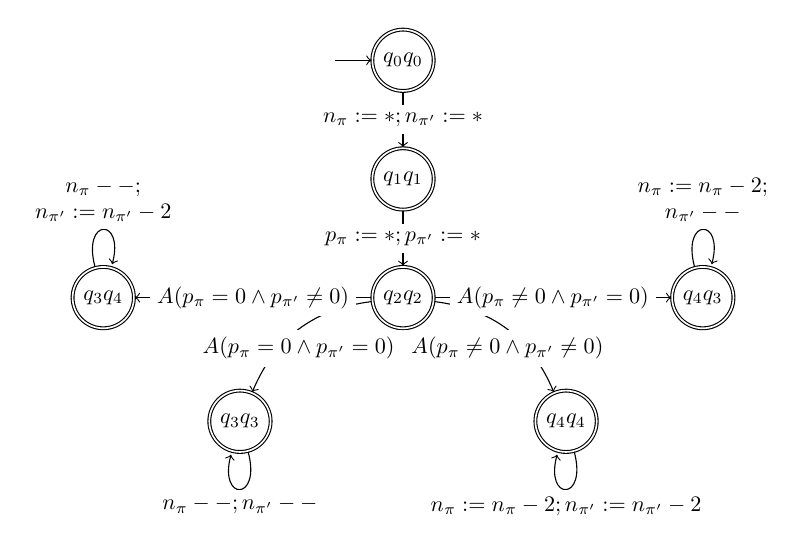
\begin{tikzpicture}[node distance = 3cm, /tikz/initial text =, every node/.style={scale=0.8, fill=white}]
    \node[state, initial, accepting] (s0s0) {$q_0q_0$};
    \node[state, accepting] (s1s1) [below =0.7cm of s0s0] {$q_1q_1$};
    \node[state, accepting] (s2s2) [below =0.7cm of s1s1] {$q_2q_2$};
    \node[state, accepting] (s3s4) [left =3cm of s2s2] {$q_3q_4$};
    \node[state, accepting] (s4s3) [right =3cm of s2s2] {$q_4q_3$};
    \node[state, accepting] (s3s3) [below left = 1cm and 1.5cm of s2s2] {$q_3q_3$};
    \node[state, accepting] (s4s4) [below right = 1cm and 1.5cm of s2s2] {$q_4q_4$};

    \path[->]
    (s0s0) edge node {$n_{\pi} := *; n_{\pi'} := *$} (s1s1)
    (s1s1) edge node {$p_{\pi} := *; p_{\pi'} := *$} (s2s2)
    (s2s2) edge [bend right=30] node [below] {$A(p_\pi = 0 \wedge p_{\pi'} = 0)$} (s3s3)
    (s2s2) edge [bend left=30] node [below] {$A(p_\pi \neq 0 \wedge p_{\pi'} \neq 0)$}  (s4s4)
    (s2s2) edge node {$A(p_\pi = 0 \wedge p_{\pi'} \neq 0)$} (s3s4)
    (s2s2) edge node {$A(p_\pi \neq 0 \wedge p_{\pi'} = 0 )$} (s4s3)
    (s3s3) edge [loop below] node {$n_\pi--; n_{\pi'}--$} ( )
    (s4s4) edge [loop below] node {$n_\pi := n_\pi-2; n_{\pi'} := n_{\pi'}-2$} ( )
    (s4s3) edge [loop above] node[align=center] {$n_\pi := n_\pi-2;$ \\ $n_{\pi'}--$} ( )
    (s3s4) edge [loop above] node[align=center] {$n_\pi--;$ \\ $n_{\pi'} := n_{\pi'}-2$} ( );

\end{tikzpicture}
\end{center}
\end{minipage}
\caption{Left: The program automaton $\aut{P}_{cy}$, Right: The program automaton $\aut{P}_{cy}^2$.}
\label{fig:cycle_example_1}
\end{figure}


The automaton 
$\aut{P}_{cy}^2$ is shown in Fig. \ref{fig:cycle_example_1}.
In the combined product, the structure of the automaton stays the same, and $\mathit{assert}(p_\pi \neq p_{\pi'} \wedge n_\pi < n_\pi')$ is added to every state. 
Removing local $k$-infeasibilities is not sufficient here; assume $k =1$. The only $1$-infeasible transition is the transition from $q_2q_2$ to $q_3q_3$, and this does not eliminate the counterexample $\pi$. Greater $k$'s do not work as well, as the remaining traces of the combined product are not $k$~infeasible for any~$k$. 


However, the self-loop at $q_3q_4$ is an infeasible accepting cycle -- the sequence \\ $(n_\pi--;~ n_{\pi'} := n_{\pi'} - 2;~ \mathit{assert} (n_{\pi} < n_{\pi'}))^\omega$ must eventually terminate. We choose $k'=1$ removing all traces ending with this cycle. Next, we project the automaton to the universal part. The trace $\pi$ is not accepted by the automaton $(\aut{P}^2 \BuechiProd \aut{A}_\psi)^\forall_{1, C(1)}$. But since $\pi$ is in $\aut{P}$ and feasible, it is identified as a counterexample.
We provide some comments on the growth conditions which constituted the majority of our analysis in sections \ref{sec:Hmixing} and \ref{sec:Hsigma}. In the simplest cases of Lemma \ref{lemma:unstableGrowth}, growth was established in an analogous fashion to the old one-step expansion condition (\ref{eq:oldOneStepExpansion}), finding the relevant Jacobians $M_j$ and checking that their expansion factors $K(M_j)$ satisfy
\begin{equation}
    \label{eq:discussionOneStep}
    \sum_j \frac{1}{K(M_j)} <1.
\end{equation}
For the more complicated cases, the inductive method used to establish growth near the accumulation points in Lemma \ref{lemma:unstableGrowth} and the weakened one-step expansion condition (\ref{eq:oneStep}) both address the same fundamental issue: the splitting of unstable curves by singularities into an unbounded number of small components. They circumvent this obstacle in rather different ways, however. While (\ref{eq:oneStep}) generalises (\ref{eq:discussionOneStep}) to ensure an growth of unstable curves `on average' (see \cite{chernov_statistical_2009} for a precise statement), our inductive method is a more direct adaptation of (\ref{eq:discussionOneStep}), using it to generate contradictory geometric conditions which a hypothetical non-growing unstable curve must satisfy. It may be possible to prove Theorem \ref{sec:Hmixing} using (\ref{eq:oneStep}) as the basis for growth. Since we required (\ref{eq:oneStep}) anyway for proving Theorem \ref{thm:HsigmaExp}, this could potentially condense our analysis, but only to a minor extent. A convenience of the method used in section \ref{sec:Hmixing} is that, by way of the `simple intersection' property, it naturally gives geometric information on the images of manifolds, useful for proving the property \textbf{(M)} of Theorem \ref{thm:katok-strelcyn}.

We expect that essentially analogous analysis can be applied to establish mixing properties in a wide class of piecewise linear non-uniformly hyperbolic maps, including those (like the OTM) which sit on the boundary of ergodicity and beyond. While we have relied on the precise partition structure of $H_\sigma$, its fundamental feature (self-similar sequences of elements $A^k$, sharing boundaries with its neighbours $A^{k-1},A^{k+1}$ and accumulating onto some point $p$) is quite typical to return map systems. See, for example, those of various stadium billiards \cite{chernov_chaotic_2006,chernov_improved_2008,chernov_statistical_2009} and LTMs \cite{springham_polynomial_2014}. Indeed, the same method can be used to prove the Bernoulli property for non-monotonic LTMs \cite{myers_hill_mixing_2022}, where monotonicity of the manifold images cannot be assumed and the classical argument \cite{sturman_mathematical_2006} fails. The OTM is the pointwise limit of these maps as the boundary shrinks to null measure. It further has utility in proving growth conditions for maps which are uniformly hyperbolic but possess regions $A_j$ where the hyperbolicity is very weak, signified by $K(M_j) \approx 1$, so that (\ref{eq:discussionOneStep}) fails. Typically this leads to suboptimal bounds on mixing windows, see e.g. \cite{wojtkowski_model_1981,przytycki_ergodicity_1983,myers_hill_family_2022}. The map $H_{(\eta,\eta)}$ for $\eta \approx 1/2$ is another example, possessing weak hyperbolicity over $A_2, A_3$. Letting $\varepsilon = |\eta-1/2|>0$, there is an upper bound $N = N(\varepsilon)$ on escape times from the intersections $A_2\cap \sigma, A_3 \cap \sigma$. The growth lemma then follows by applying the inductive step roughly $N$ times and can be established for arbitrarily small $\varepsilon$, opening the door to establishing optimal mixing windows.

The above gives two examples of piecewise linear perturbations to $H$ where mixing with respect to Lebesgue is preserved and our methods can be applied. Nonlinear perturbations to the shear profiles complicate the analysis in several ways. Firstly as the map's Jacobians takes on a broader range of values, cone invariance becomes an increasingly harder condition to establish. Cones must be widened, giving looser bounds on expansion factors, which may already be weak due to new regions of weaker stretching. This, together with the change from polygonal to curvilinear return time partition elements and nonlinear local manifolds, adds some complexity to showing growth conditions. This does not rule out certain (small) nonlinear perturbations however. There is some leeway in the inequalities which govern cone invariance and growth of local manifolds, the latter of which is not too dissimilar from the piecewise linear setting (see Lemmas \ref{lemma:piecewiseApprox}, \ref{lemma:componentLength}). Certain small perturbations would not alter the \emph{topological} structure of the return time partition, i.e. which elements share boundaries, the key information needed for setting up the induction. Finally while the partition elements would no longer be polygonal, only coarse geometric information is required for verifying each inductive step. Following the above, a potential perturbation could be to replace the linear portions of each shear by a cubic, perturbing the tent profile
\[  f(t) = \begin{cases} 2t & 0 \leq t \leq 1/2, \\ 2(1-t) & 1/2 \leq t \leq 1 ,\end{cases} \]
of the OTM shears to
\[  f_a(t) = \begin{cases} \frac{1}{8} t \left(16 - a + 6at - 8at^{2} \right) & 0 \leq t \leq 1/2, \\ \frac{1}{8}\left(1-t\right)\left( 16 - a + 6a\left(1-t\right) - 8a\left(1-t\right)^{2}\right)  & 1/2 \leq t \leq 1, \end{cases}   \]
for $a>0$. For small enough $a$ the gradient range $f'(t)$ is restricted to small neighbourhoods of $\{ 2, -2\}$ and the escape time partition retains a similar structure. We illustrate this in Figure \ref{fig:perturbations}, showing escapes from the square $S_3$ under the map $G \circ F$, equivalent to escapes from the perturbed $A_3$ under the $G \circ F$, but with a cleaner geometry for comparison. When $a$ is too large the analogy to the OTM breaks down. At $a=16$ the map is twice differentiable everywhere and features a new source of slowed mixing, the Jacobian is the identity at the corner points $x,y \in \{  0, 1/2 \}$ giving locally parabolic behaviour (visible in the escape time partition). 

\begin{figure}
    \centering
    \includegraphics[width=0.24 \linewidth]{0.png}
    \includegraphics[width=0.24 \linewidth]{4.png}
    \includegraphics[width=0.24 \linewidth]{8.png}
    \includegraphics[width=0.24 \linewidth]{16.png}
    \caption{Partition of escape times from $S_3$ under the mapping $F \circ G$ for $a= 0,4,8,16$. }
    \label{fig:perturbations}
\end{figure}

\bibliographystyle{plain}
\bibliography{thesis}

\newpage
\appendix 
\section{Detailed Correctness Proofs} \label{app:correctnessproof}
\subsection{Hyper Linear Temporal Logic (HyperLTL)}
\begin{comment}
    
\textit{Linear Temporal Logic (LTL)} is a language for specifying trace properties, that is, properties of sequences of sets of atomic propositions. Besides the standard boolean operators, LTL also includes modal operators, namely

\begin{itemize}
    \item the next-operator $\LTLnext$. $\LTLnext \varphi$ states that the formula $\varphi$ should hold in the next timestep.
    \item the eventually-operator $\LTLeventually$. $\LTLeventually \varphi$ states that $\varphi$ should hold at some timepoint in the future.
    \item the until-operator $\LTLuntil$. $\varphi \LTLuntil \psi$ states that the formula $\psi$ must hold eventually and, until this is the case, $\varphi$ must hold.
    \item the globally-operator $\LTLglobally$. $\LTLglobally \varphi$ states that $\varphi$ must hold from now on and forever.
\end{itemize}

We only treat the next-operator and the until-operator as native and derive the other operators.

\begin{definition}
    An \textbf{LTL Formula} is defined by the grammar
    \begin{align*}
        \varphi ::= a \mid \neg \varphi \mid \varphi \wedge \varphi \mid \LTLnext \varphi \mid \varphi \LTLuntil \varphi && \text{where } a \in AP
    \end{align*}
    The operators $\vee, \LTLeventually, \LTLglobally$ can be derived using the equations $\varphi \vee \psi = \neg (\neg \varphi \wedge \neg \psi)$, $\LTLeventually \varphi = true \LTLuntil \varphi$, $\LTLglobally \varphi = \neg \LTLeventually \neg \varphi$.
\end{definition}


\begin{definition}
    The \textbf{satisfaction of an LTL formula} with respect to a trace $s \in (2^{AP})^\omega$ and a time point $t$ is recursively defined by
\begin{align*}
    &t, s \lmodels a &&\Leftrightarrow a \in s_t \\
    &t, s \lmodels \neg \varphi &&\Leftrightarrow \neg (t, s \lmodels \varphi) \\
    &t, s \lmodels \varphi \wedge \psi &&\Leftrightarrow t, s \lmodels \varphi \wedge t, s \lmodels \psi \\
    &t, s \lmodels \LTLnext \varphi &&\Leftrightarrow t + 1, s \lmodels \varphi \\
    &t, s \lmodels \varphi\LTLuntil\psi &&\Leftrightarrow \exists t' \geq t.~ t', s \lmodels \psi \wedge \forall  t \leq t'' < t'.~ t'', s \lmodels \varphi
\end{align*}
We define $s \lmodels \varphi$ as $0, s \lmodels \varphi$
\end{definition}

It is well known that it is possible to translate an LTL formula into an equivalent Büchi automaton that accepts exactly the traces satisfying the LTL formula \cite{LTL_Buechi_Tut}. However, if the formula is of size $n$, the Büchi automaton might have up to $2^{\mathcal{O}(n)}$ states. The classical translation algorithm has been improved, making it faster in practice and reducing the size of the automaton \cite{LTL_Buechi, LTL_Buechi2}.

\textit{HyperLTL} \cite{HyperLTL} extends LTL with explicit trace quantification. An LTL formula has to hold for all traces of the system, so this is an implicit universal quantification. Within an HyperLTL formula, we can use multiple (different) quantifiers and thereby relate multiple traces. Every atomic proposition is now attached to a trace variable.
In the following, let $\Pi$ be a set of trace variables.
\end{comment}
Let AP be a finite set of atomic propositions and let $\Pi$ be a finite set of trace variables. Then, a {HyperLTL formula} is defined by the grammar
    \begin{align*}
        \varphi ::= a_\pi \mid \neg \varphi \mid \varphi \wedge \varphi \mid \LTLnext \varphi \mid \varphi \LTLuntil \varphi \mid \forall \pi.~ \varphi \mid \exists \pi.~ \varphi
    \end{align*}

\noindent where $a \in AP$ and $\pi \in \Pi$. 

The satisfaction of a HyperLTL formula is defined with respect to a mapping $m: \Pi \rightarrow (2^{AP})^\omega$ of trace variables to traces. For treating the quantifiers, we need the notion of extending such a mapping for a new trace variable. We define
\begin{align*}
    m[\pi \rightarrow s] (\pi) &= s \\
    m[\pi \rightarrow s] (\pi') &= m(\pi') &&\text{for } \pi \neq \pi'
\end{align*}

    The satisfaction of a HyperLTL formula with respect to a set of traces $Z \subseteq {2^{AP}}^\omega$, a mapping of trace variables to traces $m: \TraceVs \rightarrow {2^{AP}}^\omega$ and a time point $t$ is recursively defined by 
    \begin{align*}
        &Z, t, m \lmodels a_{\pi} &&\Leftrightarrow a \in m(\pi)_t \\
        &Z, t, m \lmodels \neg \varphi &&\Leftrightarrow \neg (Z, t, m \lmodels \varphi) \\
        &Z, t, m \lmodels \varphi \wedge \psi &&\Leftrightarrow Z, t, m \lmodels \varphi \wedge Z, t, m \models \psi \\
        &Z, t, m \lmodels \LTLnext \varphi &&\Leftrightarrow Z, t + 1, m \lmodels \varphi \\
        &Z, t, m \lmodels \varphi\LTLuntil\psi &&\Leftrightarrow \exists t' \geq t.~ Z, t', m \lmodels \psi \wedge \forall t \leq t'' < t'.~ Z, t'', m \lmodels \varphi \\
        &Z, t, m \lmodels \forall \pi.~\varphi &&\Leftrightarrow \forall s \in Z.~m[\pi \rightarrow s] \lmodels \varphi \\
        &Z, t, m \lmodels \exists \pi.~\varphi &&\Leftrightarrow \exists s \in Z.~m[\pi \rightarrow s] \lmodels \varphi
    \end{align*}
    We define $Z \lmodels \varphi$ as $Z, 0, \emptyset \lmodels \varphi$.

For the sepcial case in which there is only one trace quantifier, and this is a universal quantifier, we are in the fragment of LTL. 
\subsection{Similiarity of LTL and TSL}

The following lemma states an important relation between (Hyper)TSL and LTL. The LTL semantics is defined with respect to a sequence of subsets of atomic propositions, while the semantics of a TSL-formula or quantifier-free HyperTSL formula is defined with respect to a (hyper-)computation. A crucial observation for this thesis is that we can `translate' between the two -- a (hyper-)computation defines a sequence of predicate and update term subsets. For each time point, the subset contains exactly the predicate and update terms that are true now.

\begin{definition} \label{def:TSL_LTL}
    Let $\HComput \in \HAssigns^\omega, \PredSet \subseteq \HPredTerms, \USet \subseteq \HUpdTerms$. We define
    \begin{align*}
        \UPredSeq(\HComput, \PredSet, \USet)_t &= \{\HPredTerm \in \PredSet \mid t, \emptyset, \HComput \models \HPredTerm\} \cup \{\Upd{c}{\HFuncTerm{}} \in \USet \mid t, \emptyset, \HComput \models \Upd{c}{\FuncTerm{}}\} \\
        \UPredSeq(\HComput, \PredSet, \USet) &= \UPredSeq(\HComput, \PredSet, \USet)_0 ~\UPredSeq(\HComput, \PredSet, \USet)_1 ~\UPredSeq(\HComput, \PredSet, \USet)_2 \dots
    \end{align*}

    If $\PredSet$ and $\USet$ are clear from the context, we also omit these arguments.
\end{definition}

\begin{lemma} \label{lem:TSL_LTL}
    Let $t \in \mathbb{N}$. Let $\varphi$ be a HyperTSL-formula without quantifiers. Let $\PredSet \subseteq \HPredTerms, \USet \subseteq \HUpdTerms$ be the sets of predicate and update terms appearing in $\varphi$, respectively. Then
    \begin{align*}
        t, \UPredSeq(\HComput) \lmodels \varphi \Leftrightarrow t, \emptyset, \HComput \models \varphi
    \end{align*}
\end{lemma}
\begin{proof} (Lemma \ref{lem:TSL_LTL})
    Proof by structural induction over $\varphi$.
    \begin{itemize}
        \item Case $\varphi = \HPredTerm$
        \begin{align*}
            t, \UPredSeq(\HComput) \lmodels \HPredTerm \Leftrightarrow \HPredTerm \in \UPredSeq(\HComput)_t \Leftrightarrow t, \emptyset, \HComput \models \HPredTerm
        \end{align*}
        \item Case $\varphi = \Upd{c_\pi}{\HFuncTerm{}}$
        \begin{align*}
            t, \UPredSeq(\HComput) \lmodels \Upd{c_\pi}{\HFuncTerm{}} \Leftrightarrow \HPredTerm \in \UPredSeq(\HComput)_t \Leftrightarrow t, \emptyset, \HComput \models \Upd{c_\pi}{\HFuncTerm{}}
        \end{align*}
        \item Case $\varphi = \neg \psi$
        \begin{align*}
            t, \UPredSeq(\HComput) \lmodels \neg \psi \Leftrightarrow \neg(t, \UPredSeq(\HComput) \lmodels \psi) \Leftrightarrow \neg(t, \emptyset, \HComput \models \psi) \Leftrightarrow t, \emptyset, \HComput \models \neg \psi
        \end{align*}
        \item Case $\varphi = \psi \wedge \psi'$
        \begin{align*}
            & &&t, \UPredSeq(\HComput) \lmodels \psi \wedge \psi' \\
            &\Leftrightarrow &&t, \UPredSeq(\HComput) \lmodels \psi \wedge t, \UPredSeq(\HComput) \lmodels \psi' \\
            &\Leftrightarrow &&t, \emptyset, \HComput \models \psi \wedge t, \emptyset, \HComput \models \psi' \\
            &\Leftrightarrow &&t, \emptyset, \HComput \models \psi \wedge \psi'
        \end{align*}
        \item Case $\varphi = \LTLnext \psi$
        \begin{align*}
            t, \UPredSeq(\HComput) \lmodels \LTLnext \psi \Leftrightarrow t+1, \UPredSeq(\HComput) \lmodels \psi \Leftrightarrow t+1, \emptyset, \HComput \models \psi \Leftrightarrow t, \emptyset, \HComput \models \LTLnext \psi
        \end{align*}
        \item Case $\varphi = \psi \LTLuntil \psi'$
        \begin{align*}
            & &&t, \UPredSeq(\HComput) \lmodels \psi \LTLuntil \psi'\\
            & \Leftrightarrow &&\exists t' \geq t.~ t', \UPredSeq(\HComput) \lmodels \psi' \wedge \forall t \leq t'' < t'.~t'', \UPredSeq(\HComput) \lmodels \psi \\
            &\Leftrightarrow &&\exists t' \geq t.~ t', Z, \HComput \models \psi' \wedge \forall t \leq t'' < t'.~t'', Z, \HComput \models \psi \\
            &\Leftrightarrow &&t, \emptyset, \HComput \models \psi \LTLuntil \psi'
        \end{align*}       
    \end{itemize} 
    \vspace{-0.5cm}
\end{proof}

\subsection{Proof of Theorem \ref{thm:k_feasible}} \label{sec:k_feasible_proof}
\begin{proof}
    $\Rightarrow$
    Let $q_0, q_1, q_2 \dots \in Q^\omega$ be a run of $P$ on the $k$-feasible trace $\PTrace$. Then, for every $j \in \mathbb{N}$, $$e_j = ((q_j,\PTrace_{j},q_{j+1} \dots ,\PTrace_{j+k-2},q_{j+k-1}), \PTrace_{j+k-1}, (q_{j+1},\PTrace_{j+1}, \dots, q_{j+k-1},\PTrace_{j+k-1},q_{j+k}))$$ is a transition of $P_k$. Moreover, for every $k' < k$,
    $$ e_{k'} = ((q_0,s_0,q_1\dots ,\PTrace_{k'-1},q_{k'}), \PTrace_{k'}, (q_0, \PTrace_0, \dots ,q_{k'},\PTrace_{k'},q_{k'+1})) $$
    is also a transition of $P_k$. Thus, $q_0, q_1, \dots$ is accepted by $P_k$.

    $\Leftarrow$ 
    Let $\PTrace$ be a trace of $P$ accepted by $P_k$. Then, there exist states of $P$ $q_0, q_1 \dots$ such that for every $j \in \mathbb{N}$, $e_j$ from above is a transition of $P_k$. Thus, by the definition of $P_k$ for every $j$, $\PTrace_j \dots \PTrace_{j+k-1}$ is feasible. Thus, $\PTrace$ is $k$-feasible.
    \qed 
\end{proof}

\subsection{Proof of Theorem \ref{thm:BuechiProdModelChecking}} \label{sec:buechi_corr}

The main idea of the correctness proof is a construction that, given a computation $\Comput$ that matches a program trace $\PTrace$, constructs a computation matching the combined trace $\combine{\PTrace}{\UPredSeq(\Comput)}$ and vice versa ($\UPredSeq$ was defined in Definition \ref{def:TSL_LTL}). This gives us the necessary feasibility proofs. To do so, we define two operations, $\widetilde{(-)}$ and $(-)_{|\PTrace}$ that `nearly' invert each other: we have that $(\widetilde{\Comput})_{|\PTrace} = \Comput$ and if $\matches{\Comput}{\combine{\PTrace}{X}}$ for some $X$, we also have that $\widetilde{\Comput_{|\PTrace}} = \Comput$. In Lemma \ref{lem:corr1} we show that if $\matches{\Comput}{\combine{\PTrace}{X}}$ for some $X$, then $\matches{\Comput_{|\PTrace}}{\PTrace}$. In Lemma \ref{lem:corr2} we show that then, we also have that $X=\UPredSeq(\Comput_{|\PTrace})$. Lemma \ref{lem:corr3} states the other direction: if $\matches{\Comput}{\PTrace}$, then also $\matches{\widetilde{\Comput}}{\combine{\PTrace}{\UPredSeq(\Comput)}}$. Those three lemmata give us the feasibility proofs needed for the algorithm's correctness. Lemma \ref{lem:TSL_LTL} then gives the equivalence between the violation of the TSL-formula by $\Comput$ and the sequence $\UPredSeq(\Comput)$ being accepted by $A_{\neg \varphi}$, needed for reasoning about the existence of a trace $\combine{\PTrace}{\UPredSeq(\Comput)}$ in the Büchi program product.

We start with definining the operation $\widetilde{(-)}$. Let $\PTrace \in \Stmt^\omega$ and $\matches{\Comput}{\PTrace}$. We need to extend this computation to one that matches $\combine{\PTrace}{\UPredSeq(\Comput)}$. For every time point $t$, we need to introduce computation steps that match $\combine{\PTrace_t}{\UPredSeq(\Comput)_t} =$ \\
$ \mathit{save\_values}_{{\UPredSeq(\Comput)_t}};~ \PTrace_t;~\mathit{new\_inputs};~\mathit{check\_preds}_{{\UPredSeq(\Comput)_t}};~ \mathit{check\_updates}_{{\UPredSeq(\Comput)_t}}$. While executing $\mathit{save\_values}_{{\UPredSeq(\Comput)_t}}$, the values of the temporary variables are changed as required by the statements $tmp_j := \FuncTerm{j}$. When the actual statement $\PTrace_t$ is executed, the computation changes to $\Comput_t$, but still with the `old' input values and extended with values for the temporal variables. Next, when executing $\mathit{new\_inputs}$, we stepwise change the input values to those in $\Comput_t$.  Then, the assertions are executed and the computation cannot change anymore. 

In the following, we also need the notion of extending an assignment: we define $a[c \mapsto v](c) = v$ and $a[c \mapsto v](c') = a(c')$ for $c \neq c'$.

Let $\USet \subseteq \UpdTerms$ be in the following the set of update terms, and $\PredSet \subseteq \PredTerms$ the set of predicate terms appearing in the formula $\varphi$. 

\begin{definition} \label{def:adaptedComput}
    Let $\Inputs = \{i_1, \dots i_n\}$ be the set of inputs and \\ $\USet = \{\Upd{c_1}{\FuncTerm{1}}, \dots ,\Upd{c_m}{\FuncTerm{m}}\}$. Given a computation $\Comput$, we define the \textbf{adapted computation} $\widetilde{\Comput}$ as follows.
    \begin{align*}
        \Assign^{\mathit{tmp}_1}_t &:= \Comput_{t-1} [\mathit{tmp}_1 \mapsto \Eval(\FuncTerm{1}, \Comput_{t-1})] \\
        \Assign^{\mathit{tmp}_j}_t &:= \Assign^{\mathit{tmp}_{j-1}} [\mathit{tmp}_j \mapsto \Eval(\FuncTerm{j}, \Comput_{t-1})] &&\text{for } 1 < j \leq m\\
        \Assign_t &:= \Comput_t[\mathit{tmp}_1 \mapsto \Eval(\FuncTerm{1}, \Comput_{t-1}), \dots , \mathit{tmp}_m \mapsto \Eval(\FuncTerm{m}, \Comput_{t-1}),\\
        &~~~~~~~~i_1 \mapsto \Comput_{t-1}(i_1),~ \dots,~i_n \mapsto \Comput_{t-1}(i_n) ] \\
        \Assign^{i_1}_t &:= \Assign_t [i_1 \mapsto \Comput_t(i_1)] \\
        \Assign^{i_j}_t &:= \Assign^{i_{j-1}} [i_j \mapsto \Comput_t(i_j)] &&\text{for } 1 < j \leq n\\
        \widetilde{\Comput_t} &:= a^{\mathit{tmp}_1}_t \dots a^{\mathit{tmp}_m}_t~a_t~a^{i_1}_t~\dots~a^{i_n}_t~a^{i_n}_t~a^{i_n}_t \\
        \widetilde{\Comput} &:= \widetilde{\Comput_0}~ \widetilde{\Comput_1}\dots 
    \end{align*}
\end{definition}

Note that this is the only possibility to adapt a computation $\matches{\Comput}{\sigma}$ such that the result \textit{could} match $\combine{\sigma}{X}$ for any $X$.

Also note that $a_t^{i_n} = \Comput_t [tmp_1 \mapsto \Eval(\FuncTerm{1}, \Comput_{t-1}), \dots , tmp_m \mapsto \Eval(\FuncTerm{m}, \Comput_{t-1})]$.

We can also define the left inverse of this operation: reducing a computation that matches $\combine{\PTrace}{X}$ to a computation that matches $\PTrace$.

\begin{definition}
    Let $\PTrace \in \Stmt^\omega, X \in \mathcal{P}(\PredTerms \cup \UpdTerms)^\omega$ and $\matches{\Comput}{\combine{\PTrace}{X}}$. We define the \textbf{reduced computation} $\Comput_{|\sigma}$ as follows.
    \begin{align*}
        \iota(j) &:= (|\Inputs| + |\USet| + 3) \cdot (j+1) -3 \\
        \Comput_{|\PTrace}(U) &:= (\Comput_{\iota(0)})_{| (\Inputs \cup \Cells)}~(\Comput_{\iota(1)})_{| (\Inputs \cup \Cells)} \dots
    \end{align*}
    where $a_{| (\Inputs \cup \Cells)}$ means restricting the domain of the assignment to the original inputs and cells, thus excluding the temporal variables $tmp_1, tmp_2 \dots$
\end{definition}

Note that if $\matches{\Comput}{\combine{\PTrace}{X}}$, we also have that $\Comput = \widetilde{\Comput_{|\PTrace}}$, as this is the \textit{only} computation that could potentially match $\combine{\PTrace}{X}$ and equals $\Comput_{|\PTrace}$ when restricted to~$\PTrace$. 

\begin{lemma} \label{lem:corr1}
    If $\matches{\Comput}{\combine{\PTrace}{X}}$, then $\matches{\Comput_{|\PTrace}}{\sigma}$.
\end{lemma}
\begin{proof}
    We have to show that $\forall t \in \mathbb{N}.~\matchest{\Comput_{|\PTrace}}{\PTrace}{t}$

    Recall that $\Comput = \widetilde{\Comput_{|\PTrace}}$ and
    \begin{align*}
        \widetilde{(\Comput_{|\PTrace})_t} = a^{tmp_1}_t \dots a^{tmp_m}_t~a_t~a^{i_1}_t~\dots~a^{i_n}_t~a^{i_n}_t~a^{i_n}_t
    \end{align*}

    \begin{itemize}
        \item Case $\PTrace_t = \mathit{assert}(\PredTerm)$ \\
        We know that $\matchest{\Comput}{\combine{\PTrace}{X}}{\iota(t)-|\Inputs|}$. The corresponding statement is $\sigma_j$, thus
        \begin{align*}
            \Eval(\PredTerm, \Comput_{\iota(t)-|\Inputs|-1}) = true ~~~\wedge \forall c \in \Cells^*.~\Comput_{\iota(t)-|\Inputs|}(c) = \Comput_{\iota(t)-|\Inputs|-1}(c)
        \end{align*} 
        Moreover, $(\Comput_{\iota(t)-|\Inputs|-1}) = a_t^{tmp_m}$. This equals $(\Comput_{|\PTrace})_{t-1}$ extended with values for the temporary variables. As $\PredTerm$ does not contain the temporal variables, this means that $\Eval(\PredTerm, ((\Comput_{|\PTrace})_{t-1})_{|(\Inputs \cup \Cells)})$ is also true. It remains to show that             
        \begin{align*}
            \forall c \in \Cells.~(\Comput_{\iota(t-1)})_{|(\Inputs \cup \Cells)} (c) = (\Comput_{\iota(t)})_{|(\Inputs \cup \Cells)} (c)
        \end{align*}
        This is true as the only cells changed in $\Comput_{\iota(t-1)} \dots \Comput_{\iota(t)-|\Inputs|-1}$ and in $\Comput_{\iota(t) - |\Inputs|},\dots \Comput_{\iota(t)}$ are cells from $\Cells^* \backslash \Cells$.
        \item The two remaining cases are analogous.
    \end{itemize}
    \vspace{-0.5cm}
\end{proof}

\begin{lemma} \label{lem:corr2}
    If $\matches{\Comput}{combine(\PTrace, X)}$, then $X = \UPredSeq(\Comput_{|\PTrace})$.
\end{lemma}
\begin{proof}
    We prove $\forall t.~ X_t = \UPredSeq(\Comput_{|\PTrace})_t$.
    We know that $\matchest{\Comput}{\combine{\PTrace}{X}}{\iota(t)+1}$. The corresponding statement is $\mathit{check\_preds}_{X_t}$. Set $h = \left(\bigwedge_{\PredTerm \in {X_t}} \PredTerm \wedge \bigwedge_{\PredTerm \in \PredSet \backslash {X_t}} \neg \PredTerm \right)$. This means that 
    \begin{align*}
        \Eval(h, \Comput_{\iota(t)+1}) = true ~~~\wedge \forall c \in \Cells^*.~\Comput_{\iota(t)+1}(c) = \Comput_{\iota(t)}(c)
    \end{align*}
    This implies that $true = \Eval((h, \Comput_{\iota(t)})_{|(\Inputs \cup \Cells)}) = \Eval(h, (\Comput_{|\PTrace})_t)$. Therefore, for all $\PredTerm \in \PredSet$
    \begin{align*}
        \PredTerm \in \UPredSeq(\Comput_{|\PTrace})_t \Leftrightarrow t, \Comput_{|\PTrace} \models \PredTerm \Leftrightarrow \Eval(\PredTerm, \Comput_{\iota(t)}) = true \Leftrightarrow \PredTerm \in {X_t}
    \end{align*} 

    For the update terms, we know that $\matchest{\Comput}{\combine{\PTrace}{X}}{\iota(t)+2}$. The corresponding statement is $\mathit{check\_updates}_{X_t}.$ Set $h=\left( \bigwedge_{\Upd{c_j}{\FuncTerm{j}} \in \USet}
    \begin{cases}
        c_j = tmp_j &\text{if } \Upd{c_j}{\FuncTerm{j}} \in X_t\\
        c_j \neq tmp_j &\text{else} 
    \end{cases}        
        \right)$ As before, we know that $\Eval(h, (\Comput_{|\PTrace})_t) = true$. Moreover, we know that for each $j$, $(\Comput_{|\PTrace})_t (tmp_j) = \Eval(\FuncTerm{j}, (\Comput_{|\PTrace})_{t-1})$ by definition \ref{def:adaptedComput} Therefore, for every $\Upd{c_j}{\FuncTerm{j}} \in \USet,$
        \begin{align*}
            \Upd{c_j}{\FuncTerm{j}} \in \UPredSeq(\Comput_{|\PTrace})_t &\Leftrightarrow t, \Comput_{|\PTrace} \models \Upd{c_j}{\FuncTerm{j}} \\ 
            &\Leftrightarrow \Eval({\FuncTerm{j}}, \Comput_{\iota(t-1)}) = \Eval(c_j, \Comput_{\iota(t)}) \\
            &\Leftrightarrow \Eval(c_j = tmp_j, \Comput_{\iota(t)}) = true \\
            &\Leftrightarrow \Upd{c_j}{\FuncTerm{j}} \in X_t
        \end{align*}
\end{proof}

\begin{lemma} \label{lem:corr3}
    If $\matches{\Comput}{\PTrace}$, then $\matches{\widetilde{\Comput}}{\combine{\PTrace}{\UPredSeq(\Comput)}}$
\end{lemma}
\begin{proof}
    We have to show that for all $t$, $\matchest{\widetilde{\Comput}}{\combine{\PTrace}{\UPredSeq(\Comput)}}{t}$. This is clear for all time steps except for those of kind $\mathit{check\_preds}$ or $\mathit{check\_updates}$ by the definition of $\widetilde{\Comput}$.

    First consider $\mathit{check\_preds}$. We need to show that $\forall t$, $\matchest{\widetilde{\Comput}}{\combine{\PTrace}{\UPredSeq(\Comput)}}{\iota(t)+1}$. This boils down to
    \begin{align*}
        \Eval\left( \left(\bigwedge_{\PredTerm \in {\UPredSeq(\Comput)_t}} \PredTerm \wedge \bigwedge_{\PredTerm \in \PredSet \backslash {\UPredSeq(\Comput)_t}} \neg \PredTerm \right), \widetilde{\Comput}_{\iota(t)} \right) = true
    \end{align*}
    As the temporary variables $\mathit{tmp}_1, \mathit{tmp}_2 \dots $ are not used in any $\PredTerm \in \PredSet$, this is by definition \ref{def:adaptedComput} equivalent to
    \begin{align*}
        \forall \PredTerm \in \PredSet.~\PredTerm \in \UPredSeq(\Comput)_t \Leftrightarrow \Eval(\PredTerm, \Comput_t) = true
    \end{align*}
    This is true by the definition of $\UPredSeq(\Comput)_t$.

    Now consider $\mathit{check\_updates}$. We need to show that $\forall t$, $\matchest{\widetilde{\Comput}}{\combine{\PTrace}{\UPredSeq(\Comput)}}{\iota(t)+2}$. This boils down to
    \begin{align*}
        \Eval\left(\left( \bigwedge_{\Upd{c_j}{\FuncTerm{j}} \in \USet}
        \begin{cases}
            c_j = \mathit{tmp}_j &\text{if } \Upd{c_j}{\FuncTerm{j}} \in \UPredSeq(\Comput)_t\\
            c_j \neq \mathit{tmp}_j &\text{else} 
        \end{cases}        
            \right), \widetilde{\Comput}_{\iota(t)} \right) = true
    \end{align*}
    Which is equivalent to 
    \begin{align*}
        \forall \Upd{c_j}{\FuncTerm{j}} \in \USet.~ \Eval(c_j = \mathit{tmp}_j, \widetilde{\Comput}_{\iota(t)}) = true \Leftrightarrow \Upd{c_j}{\FuncTerm{j}} \in \UPredSeq(\Comput)_t
    \end{align*}
    We know that $\widetilde{\Comput}_{\iota(t)}(\mathit{tmp}_j) = \Eval(\FuncTerm{j}, \Comput_{t-1})$. Thus this is equivalent to 
    \begin{align*}
        \forall \Upd{c_j}{\FuncTerm{j}} \in \USet.~ \Eval(\FuncTerm{j}, \Comput_{t-1}) = \Comput_{t}(c) \Leftrightarrow \Upd{c_j}{\FuncTerm{j}} \in \UPredSeq(\Comput)_t
    \end{align*}
    which is again true by the definition of $\UPredSeq(\Comput)_t$.
\end{proof}

Now, we have all the lemmas needed to prove Theorem \ref{thm:BuechiProdModelChecking}
\begin{proof} (Theorem \ref{thm:BuechiProdModelChecking}) \\
    $\Rightarrow$
    Assume that $P \BuechiProd A_{\neg \varphi}$ has a feasible trace. Then, this is a trace $\combine{\PTrace}{X}$ for some $\PTrace \in \mathcal{L}(P)$ and $X \in \mathcal{L}(A_{\neg \varphi})$. Moreover, $\matches{\Comput}{\combine{\PTrace}{X}}$ for some $\Comput \in \Assigns^\omega$. By Lemma \ref{lem:corr2}, we know that $X=\UPredSeq(\Comput)$ and by Lemma \ref{lem:corr1} we know that $\matches{\Comput}{\PTrace}$. By the correctness of $A_\varphi$, we know that $\UPredSeq(\Comput) \lmodels \neg \varphi$, which by Lemma \ref{lem:TSL_LTL} means that $\Comput \models \neg \varphi$. Thus $\Comput$ is a counterexample that proves that $P$ does not satisfy $\varphi$.

    $\Leftarrow$
    Assume that $P$ does not satisfy $\varphi$. Then, there is a trace $\PTrace \in \mathcal{L}(P)$ and a computation $\Comput$ such that $\matches{\Comput}{\PTrace}$ and $\Comput \models \neg \varphi$. This means by Lemma \ref{lem:TSL_LTL} that $\UPredSeq(\Comput) \lmodels \neg \varphi$, so $\UPredSeq(\Comput)$ is accepted by $A_{\neg \varphi}$. Then, $\combine{\PTrace}{\UPredSeq(\Comput)}$ is a trace of $P \BuechiProd A_{\neg \varphi}$. By Lemma \ref{lem:corr3}, $\matches{\widetilde{\Comput}}{\combine{\PTrace}{\UPredSeq(\Comput)}}$, so this is also a feasible trace.
\end{proof}


\subsection{Proof of Theorems \ref{thm:BuechiProdModelCheckingAFH} and \ref{thm:BuechiProdModelCheckingAFH2}} \label{sec:BuechiProd_corr2}
 As the two theorems are dual, it suffices to give the proof for Theorem \ref{thm:BuechiProdModelCheckingAFH}.
 
The proof is analogous to the proof of Theorem \ref{thm:BuechiProdModelChecking}, but we have to deal with multiple traces and thus even more indices now. We give it here for completeness.

Given $n$ program traces $\PTrace_{\pi_1}, \dots \PTrace_{\pi_n}$, we define $\PTrace_j = ({(\PTrace_{\pi_1})_{\pi_1}}_j; {(\PTrace_{\pi_2})_{\pi_2}}_j; \dots {(\PTrace_{\pi_n})_{\pi_n}}_j)$ and $\PTrace = \PTrace_1 \PTrace_2 \dots$. Let $\matches{\Comput_{\pi_1}}{\PTrace_{\pi_1}} \wedge \dots \wedge \matches{\Comput_{\pi_n}}{\PTrace_{\pi_n}}$. Let $\HComput = \ExtComput{\emptyset}{\pi_1}{\Comput_{\pi_1}} \dots \ExtComput{}{\pi_n}{\Comput_{\pi_n}}$. Those computations are extendable to a computation that matches $\combine{\PTrace}{\UPredSeq(\HComput)}$ For every time point $t$, we need to introduce the computation steps that match $\combine{\PTrace_t}{X_t} = \mathit{save\_values};~\PTrace_t;~\mathit{new\_inputs};~\mathit{check\_preds}_{X_t};~ \mathit{check\_updates}_{X_t}$. While executing $\mathit{save\_values}$, the values of the relevant temporary variables are changed as required by the statements $tmp_j := \HFuncTerm{j}$. After the actual statements $\PTrace_t$ are executed, the computation changes to $\HComput_t$, but still with the `old' inputs and extended with values for the temporal variables. Next, when executing $\mathit{new\_inputs}$, we stepwise change the input values to those in $\HComput_t$. Then, the assertions are executed and the computation cannot change anymore. 

In the following, we also need the notion of extending a hyper-assignment: we define $\HAssign[c \mapsto v](c) = v$ and $\HAssign[c \mapsto v](c') = \HAssign(c')$ for $c \neq c'$.

Let $\USet \subseteq \HUpdTerms$ be in the following the set of update terms and $\PredSet \subseteq \HPredTerms$ the predicate terms appearing in the formula $\varphi$.

\begin{definition} \label{def:hadaptedComput}
    Let $\Inputs \times \TraceVs = \{i_1, \dots i_k\}$ be the set of inputs and $\USet = \{\Upd{c_1}{\HFuncTerm{1}}, \dots ,\Upd{c_m}{\HFuncTerm{m}}\}$. Given computations $\Comput_{\pi_1} \dots \Comput_{\pi_n}$, let $\HComput = \ExtComput{\emptyset}{\pi_1}{\PTrace_{\pi_1}} \dots \ExtComput{}{\pi_n}{\PTrace_{\pi_n}}$. We define the \textbf{adapted computation} $\widetilde{(\Comput_{\pi_1}, \dots ,\Comput_{\pi_n})}$.
    \begin{align*}
        \HAssign^{\mathit{tmp}_1}_t &:= \HComput_{t-1} [\mathit{tmp}_1 \mapsto \Eval(\FuncTerm{1},\HComput_{t-1})] \\
        \HAssign^{\mathit{tmp}_j}_t &:= \HAssign^{\mathit{tmp}_{j-1}} [\mathit{tmp}_j \mapsto \Eval(\FuncTerm{j},\HComput_{t-1})] ~~~~~~~~~~~~~~~~~~~\text{for } 1 < j \leq m\\
        \HAssign^{\pi_j}_t &= (\HComput_{t-1}\ExtComput{}{\pi_1}{\Comput_{\pi_1}} \dots \ExtComput{}{\pi_j}{\Comput_{\pi_j}})_t
         [i_1 \mapsto \Comput_{t-1}(i_1),~\dots~,i_k \mapsto \Comput_{t-1}(i_k), \\
         &~~~~\mathit{tmp}_1 \mapsto \Eval(\FuncTerm{1},\HComput_{t-1}), \dots , \mathit{tmp}_m \mapsto \Eval(\FuncTerm{m},\HComput_{t-1})] \\
         \HAssign^{i_1}_t &:= \HAssign_t^{\pi_n} [i_1 \mapsto \HComput_t(i_1)] \\
        \HAssign^{i_j}_t &:= \HAssign^{i_{j-1}} [i_j \mapsto \HComput_t(i_j)] ~~~~~~~~~~~~~~~~~~~~~~~~~~~~\text{for } 1 < j \leq k\\
         \widetilde{(\Comput_{\pi_1}, \dots ,\Comput_{\pi_n})^t} &:= \HAssign^{\mathit{tmp}_1}_t \dots \HAssign^{\mathit{tmp}_n}_t ~\HAssign^{\pi_1}_t \dots \HAssign^{\pi_n}_t~\HAssign^{i_1}_t~\dots~\HAssign^{i_k}_t~\HAssign^{i_k}_t~\HAssign^{i_k}_t \\
         \widetilde{(\Comput_{\pi_1}, \dots ,\Comput_{\pi_n})} &:= \widetilde{(\Comput_{\pi_1}, \dots ,\Comput_{\pi_n})^0}~ \widetilde{(\Comput_{\pi_1}, \dots ,\Comput_{\pi_n})^1}\dots 
    \end{align*}
\end{definition}

Note that this is the only possibility to extend the computations $\matches{\Comput_{\pi_1}}{\PTrace_{\pi_1}}, \dots, \matches{\Comput_{\pi_n}}{\PTrace_{\pi_n}}$ to a computation that potentially matches $\combine{\PTrace}{X}$ for any $X$.

We can also define the left inverse of this operation: reducing a computation that matches $\combine{\PTrace}{X}$ to computations that match $\PTrace_{\pi_1}, \dots , \PTrace_{\pi_n}$ as follows.

\begin{definition}
    Let $1 \leq j \leq n, \PTrace \in \Stmt^\omega, X \in \mathcal{P}(\HPredTerms \cup \HUpdTerms)^\omega$ and $\matches{\HComput}{\combine{\PTrace}{X}}$.
    We define the index of the computation step of $(\PTrace_{\pi_{j}})_t$ in $\combine{\PTrace}{X}$
    \begin{align*}
        \iota(t) &:= (|\Inputs \times \TraceVs| + |\USet| + n + 2) \cdot (t+1) - 3
    \end{align*}
    We define the \textbf{reduced computation} $\Comput_{|\pi_j}$.
    \begin{align*}
        \Comput_{|\pi_j} &:= (\Comput_{\iota(0)})_{| (\Inputs \cup \Cells)_{\pi_j}} ~(\Comput_{\iota(1)})_{| (\Inputs \cup \Cells)_{\pi_j}} \dots
    \end{align*}
    where $\HAssign_{| (\Inputs \cup \Cells)_{\pi_j}}$ means restricting the domain of the assignment to the cells and inputs labeled with $\pi_j$, thus excluding the temporal variables $tmp_1, tmp_2 \dots$ and the variables from other traces. Moreover, the cells and inputs are again renamed from $c_{\pi_j}$ to $c$ or $i_{\pi_j}$ to $i$.
\end{definition}

Note that if $\matches{\HComput}{\combine{\PTrace}{X}}$, we also have that $\HComput$ is the adapted computation of $(\HComput_{|\pi_1}, \dots ,\HComput_{|\pi_n})$ as this is the \textit{only} computation that could match $\combine{\PTrace}{X}$ and equals $\Comput_{|\pi_j}$ when restricted to $\pi_j$. 

\begin{lemma} \label{lem:hcorr1}
    If $\matches{\HComput}{\combine{\PTrace}{X}}$ and $\PTrace = ((\PTrace_{\pi_1})_{\pi_1}, \dots ,(\PTrace_{\pi_n})_{\pi_n})$, then $\matches{\HComput_{|\pi_j}}{\PTrace_{\pi_j}}$ for every $1 \leq j \leq n$.
\end{lemma}
\begin{proof}
    We show that $\forall t \in \mathbb{N}. ~\matchest{\HComput_{|\pi_j}}{\PTrace_{\pi_j}}{t}$.

    Recall that $\HComput$ is the adapted computation of $(\HComput_{|\pi_1}, \dots ,\HComput_{|\pi_n})$ .

    \begin{itemize}
        \item Case $\PTrace_{t} = \mathit{assert}(\PredTerm)$ \\
        We know that $\matchest{\HComput}{\combine{\PTrace}{X}}{\iota(t) - |\Inputs \times \TraceVs| - (n-j)}$, and  thus
        \begin{align*}
            &\Eval(\HPredTerm, \HComput_{\iota(t)-|\Inputs \times \TraceVs|-(n-j)-1}) = true~~ \wedge \\ &\forall c \in \Cells^*.~\HComput_{\iota(t)-|\Inputs \times \TraceVs| - (n-j)}(c) = \HComput_{\iota(t)-|\Inputs \times \TraceVs|(n-j)-1}(c)
        \end{align*} 
        Moreover, $(\HComput_{\iota(t)-|\Inputs \times \TraceVs|-(n-j)-1})$ equals $\HAssign^{tmp_m}_t$ if $j=0$ and else $\HAssign^{\pi_{j-1}}_t$, which both equals $(\HComput_{|\pi_j})_{t-1}$ when restricted to the inputs and variables from $\pi_j$. $\PredTerm$ does not contain variables from other traces or temporary variables, thus $\Eval(\PredTerm, (\HComput_{|\pi_j})_{t-1})$ is also true. It remains to show that             
        \begin{align*}
            \forall c \in \Cells.~((\HComput)_{\iota(t-1)})_{|(\Inputs \cup \Cells)_{\pi_j}} (c) = ((\HComput)_{\iota(t)})_{|(\Inputs \cup \Cells)_{\pi_j}} (c)
        \end{align*}
        This is also true as the only cells changed in $\HComput_{\iota(t-1)} \dots \HComput_{\iota(t)-|\Inputs \times \TraceVs|-(n-j)-1}$ and in $\HComput_{\iota(t)-(n-j)-|\Inputs \times \TraceVs|}, \dots \HComput_{\iota(t)}$ are cells from $\Cells^* \backslash \Cells$ or cells from other traces.
        \item The two remaining cases are analogous.
    \end{itemize}
\end{proof}

\newcommand{\longseq}{\UPredSeq(\emptyset \ExtComput{}{\pi_1}{\HComput_{|\pi_1}} \dots \ExtComput{}{\pi_n}{\HComput_{|\pi_n}} )}


\begin{lemma} \label{lem:hcorr2}
    If $\matches{\HComput}{combine(\PTrace, X)}$, then $X = \longseq$ 
\end{lemma}
\begin{proof}
    Set $\HComput' = \emptyset \ExtComput{}{\pi_1}{\HComput_{|\pi_1}} \dots \ExtComput{}{\pi_n}{\HComput_{|\pi_n}}$. We prove $\forall t.~ X_t = \UPredSeq(\HComput')_t$.
    We know that $\matchest{\HComput}{\combine{\PTrace}{X}}{\iota(t)+1}$. The corresponding statement is $check\_preds_{X_t}$. Set $h = \left(\bigwedge_{\PredTerm \in {X_t}} \HPredTerm \wedge \bigwedge_{\HPredTerm \in \PredSet \backslash {X_t}} \neg \PredTerm \right)$. This means that 
    \begin{align*}
        \Eval(h, \HComput_{\iota(t)+1}) = true ~~~\wedge \forall c \in \Cells^*.~\Comput_{\iota(t)+1}(c) = \HComput_{\iota(t)}(c)
    \end{align*}

    Recall that $\HComput_{\iota(t)+1}$ is by Definition \ref{def:hadaptedComput} equal to
    \begin{align*}
        &(\HComput'_{t-1}\ExtComput{}{\pi_1}{\HComput'_{\pi_1}} \dots \ExtComput{}{\pi_j}{\HComput'_{\pi_n}})_t~
         [\mathit{tmp}_1 \mapsto \Eval(\HFuncTerm{1}, \HComput'_{t-1}), \dots , \mathit{tmp}_m \mapsto \Eval(\HFuncTerm{m}, \HComput'_{t-1})] \\
         &=  \HComput'_t~
         [\mathit{tmp}_1 \mapsto \Eval(\HFuncTerm{1}, \HComput'_{t-1}), \dots , \mathit{tmp}_m \mapsto \Eval(\HFuncTerm{m}, \HComput'_{t-1})]
    \end{align*}
    $h$ does not contain the temporal variables, so this implies that $\Eval(h, \HComput'_t) = true$. Therefore, for all $\PredTerm \in P$
    \begin{align*}
        \PredTerm \in \UPredSeq(\HComput')_t \Leftrightarrow t, \HComput' \models \PredTerm \Leftrightarrow \Eval(\PredTerm, \Comput'_t) = true \Leftrightarrow \PredTerm \in {X_t}
    \end{align*} 
    The last equivalence holds by the definition of $h$.

    For the update terms, we know that $\matchest{\Comput}{\combine{\PTrace}{X}}{\iota(t)+2}$. The corresponding statement is $\mathit{check\_updates}_{X_t}$. Set $h=\left( \bigwedge_{\Upd{c_j}{\HFuncTerm{j}} \in \USet}
    \begin{cases}
        c_j = \mathit{tmp}_j &\text{if } \Upd{c_j}{\HFuncTerm{j}} \in X_t\\
        c_j \neq \mathit{tmp}_j &\text{else} 
    \end{cases}        
        \right)$ As before, we know that $\Eval(h, \HComput'_t) = true$. Moreover, we know that for each $j$, $\HComput_{\iota(t)+1} (\mathit{tmp}_j) = \Eval(\HFuncTerm{j},\HComput'_{t-1})$ again by Definition \ref{def:hadaptedComput} Therefore, for every $\Upd{c_j}{\HFuncTerm{j}} \in \USet,$
        \begin{align*}
            \Upd{c_j}{\HFuncTerm{j}} \in \UPredSeq(\HComput')_t &\Leftrightarrow t, \HComput' \models \Upd{c_j}{\HFuncTerm{j}} \\ 
            &\Leftrightarrow \Eval({\HFuncTerm{j}}, \HComput'_{t-1}) = \Eval(c_j, \HComput'_t) \\
            &\Leftrightarrow \Eval(c_j = tmp_j, \HComput'_t) = true \\
            &\Leftrightarrow \Upd{c_j}{\HFuncTerm{j}} \in X_t
        \end{align*}
        The last equivalence is again true by the definition of $h$.
\end{proof}

\begin{lemma} \label{lem:hcorr3}
    If $\matches{\Comput_{\pi_1}}{\PTrace_{\pi_1}} \wedge \dots \wedge \matches{\Comput_{\pi_n}}{\PTrace_{\pi_n}}$, then $\matches{\widetilde{(\Comput_{\pi_1}, \dots ,\Comput_{\pi_n})}}{\combine{\PTrace}{\UPredSeq(\HComput')}$, where $\HComput' = \ExtComput{\emptyset}{\pi_1}{\Comput_{\pi_1}} \dots \ExtComput{}{\pi_n}{\Comput_{\pi_n}}}$
\end{lemma}
\begin{proof}
    Set $\HComput = \widetilde{(\Comput_{\pi_1}, \dots ,\Comput_{\pi_n})}$. We have to show that for all $t$, $\matchest{\HComput}{\combine{\PTrace}{\UPredSeq(\HComput')}}{t}$. This is clear for all time steps except for those of kind $\mathit{check\_preds}$ or $\mathit{check\_updates}$ by the definition of $\HComput$.

    First consider $\mathit{check\_preds}$. We need to show that $\forall t$, $\matchest{\HComput}{\combine{\PTrace}{\UPredSeq(\HComput')}}{\iota(t)+1}$. This boils down to
    \begin{align*}
        \Eval\left( \left(\bigwedge_{\HPredTerm \in {\UPredSeq(\HComput')_t}} \HPredTerm \wedge \bigwedge_{\HPredTerm \in \PredSet \backslash {\UPredSeq(\HComput')_t}} \neg \HPredTerm \right), \HComput_{\iota(t)+1} \right) = true
    \end{align*}

    Recall that $\HComput_{\iota(t)+1}$ is by Definition \ref{def:hadaptedComput} equal to
    \begin{align*}
        &(\HComput'_{t-1}\ExtComput{}{\pi_1}{\HComput'_{\pi_1}} \dots \ExtComput{}{\pi_j}{\HComput'_{\pi_n}})_t~
         [\mathit{tmp}_1 \mapsto \Eval(\HFuncTerm{1},\HComput'_{t-1}), \dots , \mathit{tmp}_m \mapsto \Eval(\HFuncTerm{m}, \HComput_{t-1})] \\
         &= \HComput'_t~ [\mathit{tmp}_1 \mapsto \Eval(\HFuncTerm{1},\HComput'_{t-1}), \dots , \mathit{tmp}_m \mapsto \Eval(\HFuncTerm{m}, \HComput_{t-1})] 
    \end{align*}

    Thus, as the temporary variables are not used in $\HPredTerm$, this is equivalent to
    \begin{align*}
        \forall \HPredTerm \in \PredSet.~\HPredTerm \in \UPredSeq(\Comput')_t \Leftrightarrow \Eval((\HPredTerm), \Comput'_t ) = true
    \end{align*}
    This is true by the definition of $\UPredSeq(\Comput)_t$.

    Now consider $\mathit{check\_updates}$. We need to show that $\forall t$, $\matchest{\HComput}{\combine{\PTrace}{\UPredSeq(\HComput')}}{\iota(t)+2}$. This boils down to
    \begin{align*}
        \Eval\left(\left( \bigwedge_{\Upd{c_j}{\HFuncTerm{j}} \in \USet}
        \begin{cases}
            c_j = \mathit{tmp}_j &\text{if } \Upd{c_j}{\HFuncTerm{j}} \in \UPredSeq(\HComput')_t\\
            c_j \neq \mathit{tmp}_j &\text{else} 
        \end{cases}        
            \right), \HComput_{\iota(t)+2} \right) = true
    \end{align*}
    Which is again equivalent to 
    \begin{align*}
        \forall \Upd{c_j}{\FuncTerm{j}} \in \USet.~ \Eval(c_j = \mathit{tmp}_j, \HComput_{\iota(t)+2}) = true \Leftrightarrow \Upd{c_j}{\FuncTerm{j}} \in \UPredSeq(\HComput')_t
    \end{align*}
    We know that $\HComput_{\iota(t)+2}(\mathit{tmp}_j) = \HComput'_{t-1}(\FuncTerm{j})$. Thus this is equivalent to 
    \begin{align*}
        \forall \Upd{c_j}{\HFuncTerm{j}} \in \USet.~ \Eval(\HFuncTerm{j}, \HComput'_{t-1}) = \HComput'_{t}(c) \Leftrightarrow \Upd{c_j}{\HFuncTerm{j}} \in \UPredSeq(\HComput')_t
    \end{align*}
    Which is again true by the definition of $\UPredSeq(\HComput')_t$.
\end{proof}

Now, we have all the lemmas needed to prove Theorem \ref{thm:BuechiProdModelCheckingAFH}
\begin{proof} (Theorem \ref{thm:BuechiProdModelCheckingAFH}) \\
    $\Rightarrow$
    Assume that $P^n \BuechiProd A_{\neg \varphi}$ has a feasible trace. Then, this is a trace $\combine{\PTrace}{X}$ for some $\PTrace \in \mathcal{L}(P^n)$ and $X \in \mathcal{L}(A_{\neg \varphi})$. We know that $\PTrace_t = ({(\PTrace_{\pi_1})_{\pi_1}}_t; \dots ;{(\PTrace_{\pi_n})_{\pi_n}}_t)$. Moreover, $\matches{\HComput}{\combine{\PTrace}{X}}$ for some $\HComput \in \HAssigns^\omega$. By Lemma \ref{lem:hcorr1}, we know that $\matches{\HComput_{|\pi_1}}{\PTrace_{\pi_1}} \wedge \dots \wedge \matches{\HComput_{|\pi_n}}{\PTrace_{\pi_n}}$. Set $\HComput' = \ExtComput{\emptyset}{\pi_1}{\HComput_{|\pi_1}} \dots \ExtComput{}{\pi_n}{\HComput_{|\pi_n}}$. By Lemma \ref{lem:hcorr2}, we know that $X=\UPredSeq(\HComput')$. By the correctness of $A_\psi$ this means that $\UPredSeq(\HComput') \lmodels \neg \varphi$ which by Lemma \ref{lem:TSL_LTL} means that $\HComput' \models \neg \varphi$. Thus, $\HComput_{|\pi_1} \dots \HComput_{|\pi_n}$ are feasible counterexample traces proving that $\forall \pi_1.~ \dots \forall \pi_n.~ \psi$ does not hold.

    $\Leftarrow$
    Assume that $P$ does not satisfy $\varphi$. Then, there are trace $\PTrace_{\pi_1}, \dots \PTrace_{\pi_n} \in \mathcal{L}(P)$ and computations $\Comput_{\pi_1}, \dots \Comput_{\pi_n}$ such that $\matches{\Comput_{\pi_1}}{\PTrace_{\pi_1}} \wedge \dots \wedge \matches{\Comput_{\pi_n}}{\PTrace_{\pi_n}}$ and \\ $\HComput' = \ExtComput{\emptyset}{\pi_1}{\Comput_{\pi_1}} \dots \ExtComput{}{\pi_n}{\Comput_{\pi_n}} \models \neg \varphi$. This means by Lemma \ref{lem:TSL_LTL} that $\UPredSeq(\HComput') \lmodels \neg \varphi$, so $\UPredSeq(\HComput')$ is accepted by $A_{\neg \varphi}$. Set $\PTrace_t = ({(\PTrace_{\pi_1})_{\pi_1}}_t; \dots ;~{(\PTrace_{\pi_n})_{\pi_n}}_t)$ and $\PTrace = \PTrace_0 \PTrace_1 \dots$. Then, $\combine{\PTrace}{\UPredSeq(\Comput)}$ is a trace of $P \BuechiProd A_{\neg \varphi}$. By Lemma \ref{lem:hcorr3}, $\matches{\widetilde{(\Comput_{\pi_1}, \dots, \Comput_{\pi_n})}}{\combine{\PTrace}{\UPredSeq(\Comput')}}$, so this is also a feasible trace.

\end{proof}

\subsection{Proof of Theorem \ref{thm:corr_AE}} \label{sec:corr_AE}

We now prove Theorem \ref{thm:corr_AE}. To do that, we need the following lemma: recall that for a program execution $\sigma_{\pi}$, $(\sigma_{\pi})_{\pi}$ means renaming every cell $c$ in $\sigma_\pi$ to $c_\pi$ and every input $i$ to $i_\pi$.

\begin{lemma} \label{lem:splittrace}
    Let $\PTrace \in \Stmt^\omega$ be feasible and $\PTrace_t = (((\PTrace_{\pi_1})_{\pi_1})_t, \dots , ((\PTrace_{\pi_n})_{\pi_n})_t )$ for some $\sigma_{\pi_1}, \dots \sigma_{\pi_n}$. Then $\PTrace_{\pi_1}, \dots, \PTrace_{\pi_n}$ are also all feasible.
\end{lemma}
\begin{proof}
    As $\PTrace$ is feasible, we know that $\matches{\HComput}{\PTrace}$ for some $\HComput$. For all $1 \leq j \leq n$, we define $\Comput_{\pi_j}$ by
    \begin{align*}
        (\Comput_{\pi_j})_t &= (\HComput_{t \cdot n + j - 1})_{|(\Inputs \cup \Cells)_{\pi_j}} \\
        \Comput_{\pi_j} &= (\Comput_{\pi_j})_0~(\Comput_{\pi_j})_1 \dots
    \end{align*}
    where $\HAssign_{| (\Inputs \cup \Cells)_{\pi_j}}$ as before means restricting the domain of the assignment to the cells and inputs labeled with $\pi_j$, thus excluding the variables from other traces. Moreover, the cells and inputs are again renamed from $c_{\pi_j}$ to $c$ or $i_{\pi_j}$ to $i$. $t \cdot m + j - 1$ is the index of $(\PTrace_{\pi_j})_t$ in $\PTrace$.
    
    We show that for all time points $t$, $\matchest{\Comput_{\pi_j}}{\PTrace_{\pi_j}}{t}$
    \begin{itemize}
        \item Case $(\Comput_{\pi_j})_t = \mathit{assert}(\PredTerm)$ \\
                We know that $\matchest{\HComput}{\PTrace}{t \cdot m + j - 1}$ and thus 
                \begin{align*}
                    \Eval(\HPredTerm, \HComput_{t \cdot m + j - 1}) = true \wedge \forall c \in \Cells \times \TraceVs.~\HComput_{t \cdot m + j - 1}(c) = \HComput_{t \cdot m + j - 2}.
                \end{align*}
                Moreover $\Eval(\PredTerm, (\Comput_{\pi_j})_t)$ is also true as $\PredTerm$ does not contain variables from other traces. It remains to show that 
                \begin{align*}
                    \forall c \in \Cells.~((\Comput_{\pi_j})_t)(c) = (\Comput_{\pi_j})_{t-1}(c)
                \end{align*}

                This is also true as the only cells changed in $\HComput_{(t-1) \cdot m + j - 1}, \dots \HComput_{t \cdot m + j - 2}$ are cells from other traces.
        \item The remaining two cases are analogous.
    \end{itemize}
\end{proof}

We now prove Theorem \ref{thm:corr_AE}
\begin{proof}
    Assume that $P^m \backslash (P^n \BuechiProd A_\psi)_{k, C(k')}^\forall$ has a feasible trace $\PTrace$ with $\matches{\HComput}{\PTrace}$. By Lemma \ref{lem:splittrace}, this means that $\matches{\Comput_{\pi_1}}{\PTrace_{\pi_1}} \wedge \dots \wedge \matches{\Comput_{\pi_m}}{\PTrace_{\pi_m}}$. It suffices to show that $\emptyset \ExtComput{}{\pi_1}{\Comput_1} \dots \ExtComput{}{\pi_m}{\Comput_m} \nmodels \exists \pi_{m+1}.~ \dots \exists \pi_n.~\psi$ as this implies that $\Comput_1, \dots \Comput_m$ are a counterexample proving that $P$ does not satifsfy $\varphi$.

    Proof by contradiction. Assume that $\emptyset \ExtComput{}{\pi_1}{\Comput_1} \dots \ExtComput{}{\pi_m}{\Comput_m} \models \exists \pi_{m+1}.~ \dots \exists \pi_n.~\psi$. Then, there are traces $\PTrace_{\pi_{m+1}}, \dots \PTrace_{\pi_n}$ and computations $\Comput_{\pi_{m+1}} \dots \Comput_{\pi_n}$ such that $\matches{\Comput_{\pi_{m+1}}}{\PTrace_{\pi_{m+1}}} \wedge \dots \wedge \matches{\Comput_{\pi_n}}{\PTrace_{\pi_n}}$ and $\HComput' = \emptyset \ExtComput{}{\pi_1}{\Comput_{\pi_1}} \dots \ExtComput{}{\pi_n}{\Comput_{\pi_n}} \models \psi$.\\ Set $\PTrace'_t = ({(\PTrace_{\pi_1})_{\pi_1}}_t; \dots ;{(\PTrace_{\pi_n})_{\pi_n}}_t)$ and $\PTrace' = \PTrace'_0~\PTrace'_1 \dots$. Now, by Lemma \ref{lem:TSL_LTL} and the correctness of $A_\psi$, we know that $\UPredSeq(\HComput')$ is accepted by $A_\psi$, thus $\combine{\PTrace'}{ \UPredSeq(\HComput')}$ is accepted by $P^n \BuechiProd A_{\psi}$. Moreover, by Lemma \ref{lem:hcorr2}, we know that $\combine{\PTrace'}{\UPredSeq(\HComput')}$ is also feasible, so it is also $k$-feasible and thus accepted by $(P^n \BuechiProd A_\psi)_k$. Moreover, does not end with an infeasible cycle and is thus also accepted by $(P^n \BuechiProd A_\psi)_{k, C(k')}$  But this means that $\PTrace$ is accepted by $(P^n \BuechiProd A_\psi)^\forall_{k, C(k')}$. and thus not by $P^m \backslash (P^n \BuechiProd A_\psi)^\forall_{k, C(k')}$. Contradiction.
\end{proof}
\end{document}
